\documentclass[10pt,twocolumn,letterpaper]{article}
\usepackage[T1]{fontenc}
\usepackage[utf8]{inputenc}
\usepackage{mathptmx}
\usepackage{amsmath}
\usepackage{graphicx}
\usepackage{array}
\usepackage{float}
\usepackage{balance}
\usepackage{cite}
\usepackage[top=0.75in,bottom=1in,left=0.625in,right=0.625in,columnsep=0.25in]{geometry}
\usepackage{titlesec}
\usepackage[font=footnotesize]{caption}
\usepackage{microtype}
\usepackage[hidelinks]{hyperref}
\graphicspath{{figures/}}
\renewcommand{\topfraction}{0.95}\renewcommand{\bottomfraction}{0.9}\renewcommand{\textfraction}{0.03}\renewcommand{\floatpagefraction}{0.8}
\renewcommand{\dbltopfraction}{0.95}\renewcommand{\dblfloatpagefraction}{0.8}
\renewcommand{\thesection}{\Roman{section}}
\renewcommand{\thesubsection}{\thesection-\Alph{subsection}}
\titleformat{\section}{\centering\normalsize\scshape}{\Roman{section}.}{0.5em}{}
\titleformat{\subsection}{\normalsize\itshape}{\Alph{subsection}.}{0.5em}{}
\titlespacing*{\section}{0pt}{10pt}{5pt}
\titlespacing*{\subsection}{0pt}{8pt}{3pt}
\captionsetup[figure]{name=Fig.,labelsep=period,justification=justified,singlelinecheck=false}
\renewcommand{\thetable}{\Roman{table}}
\captionsetup[table]{name=TABLE,labelsep=newline,justification=centering,textfont=sc}
\setlength{\tabcolsep}{3pt}
\pagestyle{plain}

\begin{document}

\twocolumn[
\begin{center}
{\fontsize{22}{26}\selectfont Fire and Smoke Image Classification Using Adaptive Digital Image Processing and a Lightweight Vision Transformer\par}
\vspace{14pt}
{\large Mahdia Hossain\par}
\vspace{2pt}
{\normalsize\itshape Department of Computer Science and Engineering \\
University of Liberal Arts Bangladesh (ULAB) \\
Dhaka, Bangladesh \\
CSE 4462 Digital Image Processing Lab, Open-Ended Lab\par}
\end{center}
\vspace{12pt}
]

\noindent\textbf{\textit{Abstract}---Fires cause great damage when they are found late. Cameras can help, but camera photos are often noisy, and many normal things look like fire or smoke. This paper presents a system that looks at one photo and says fire, smoke or normal. The system first measures the noise in the photo with the Immerkær noise estimate. It applies a 3 $\times$ 3 median filter and CLAHE on the lightness channel only when the noise level $\sigma$ is above 2.56. Clean photos are not changed. A small vision transformer, MobileViT-XS, then classifies the photo. The model is trained with added Gaussian noise. We built a clean dataset of 41,789 photos from three public sources and a separate set of 451 look-alike photos such as sunsets, lamps and fog. We trained 16 classifiers and chose the final one by validation score only. The final model reaches a macro-F1 of 0.917 on validation, 0.895 on the in-domain test set and 0.900 on a test set from a new source. It gives false alarms on only 2.2\% of the look-alike photos. Under added noise, blur, darkness and JPEG damage its macro-F1 stays at 0.81 or higher, while the same network trained on raw photos falls to 0.40. The system is released as a small Python package that shows every intermediate step.}

\vspace{4pt}
\noindent\textbf{\textit{Index Terms}---fire detection, smoke detection, digital image processing, noise estimation, median filter, CLAHE, MobileViT, robustness}


\section{Introduction}
Fires in homes, factories, streets and forests cause great damage when they are found late. Cameras are already in many places. A program that checks camera photos can raise an early alarm \cite{muhammad}.

The task in this work is simple to state. The input is one colour photo. The output is one of three classes: fire, smoke or normal. The task is hard for three reasons. First, many normal things look like fire or smoke. Sunsets, lamps and car lights look like fire. Fog and steam look like smoke. Second, real camera photos are often noisy, dark, blurred or heavily compressed. Deep networks lose accuracy on such photos \cite{dodge,hendrycks}. Third, a model must also work on photos from places it did not see in training.

Digital image processing (DIP) gives classic tools for these problems. A median filter removes noise dots \cite{huang}. CLAHE improves local contrast \cite{clahe}. But a filter also removes some real detail. If we filter every photo, clean photos lose detail for no reason.

Our idea is to filter a photo only when it needs it. The system measures the noise level of each photo with the Immerkær estimate \cite{immerkaer}. If the noise is above a threshold, the photo gets a median filter and CLAHE. If not, the photo is left unchanged. A small vision transformer, MobileViT-XS \cite{mobilevit}, then classifies the photo. We call this final model CA. Fig. \ref{fig:pipeline} shows the full pipeline.

The main contributions of this work are:

\begin{itemize}
  \item A clean dataset of 41,789 photos built from three public sources, with copies and test leaks removed, and a hand-checked set of 451 look-alike photos.
  \item A step-by-step study of the DIP steps (filters, contrast methods, colour segmentation, morphology and noise estimation), measured with PSNR, SSIM and other scores.
  \item An adaptive DIP preprocessing rule that filters only noisy photos, combined with noise training of MobileViT-XS.
  \item A fair comparison of 16 classifiers, chosen by validation score only, and a robustness test with nine kinds of image damage.
  \item A small Python package, firesmoke, that runs the model on a new photo and saves every intermediate step.
\end{itemize}

\begin{figure*}[!t]
  \centering
  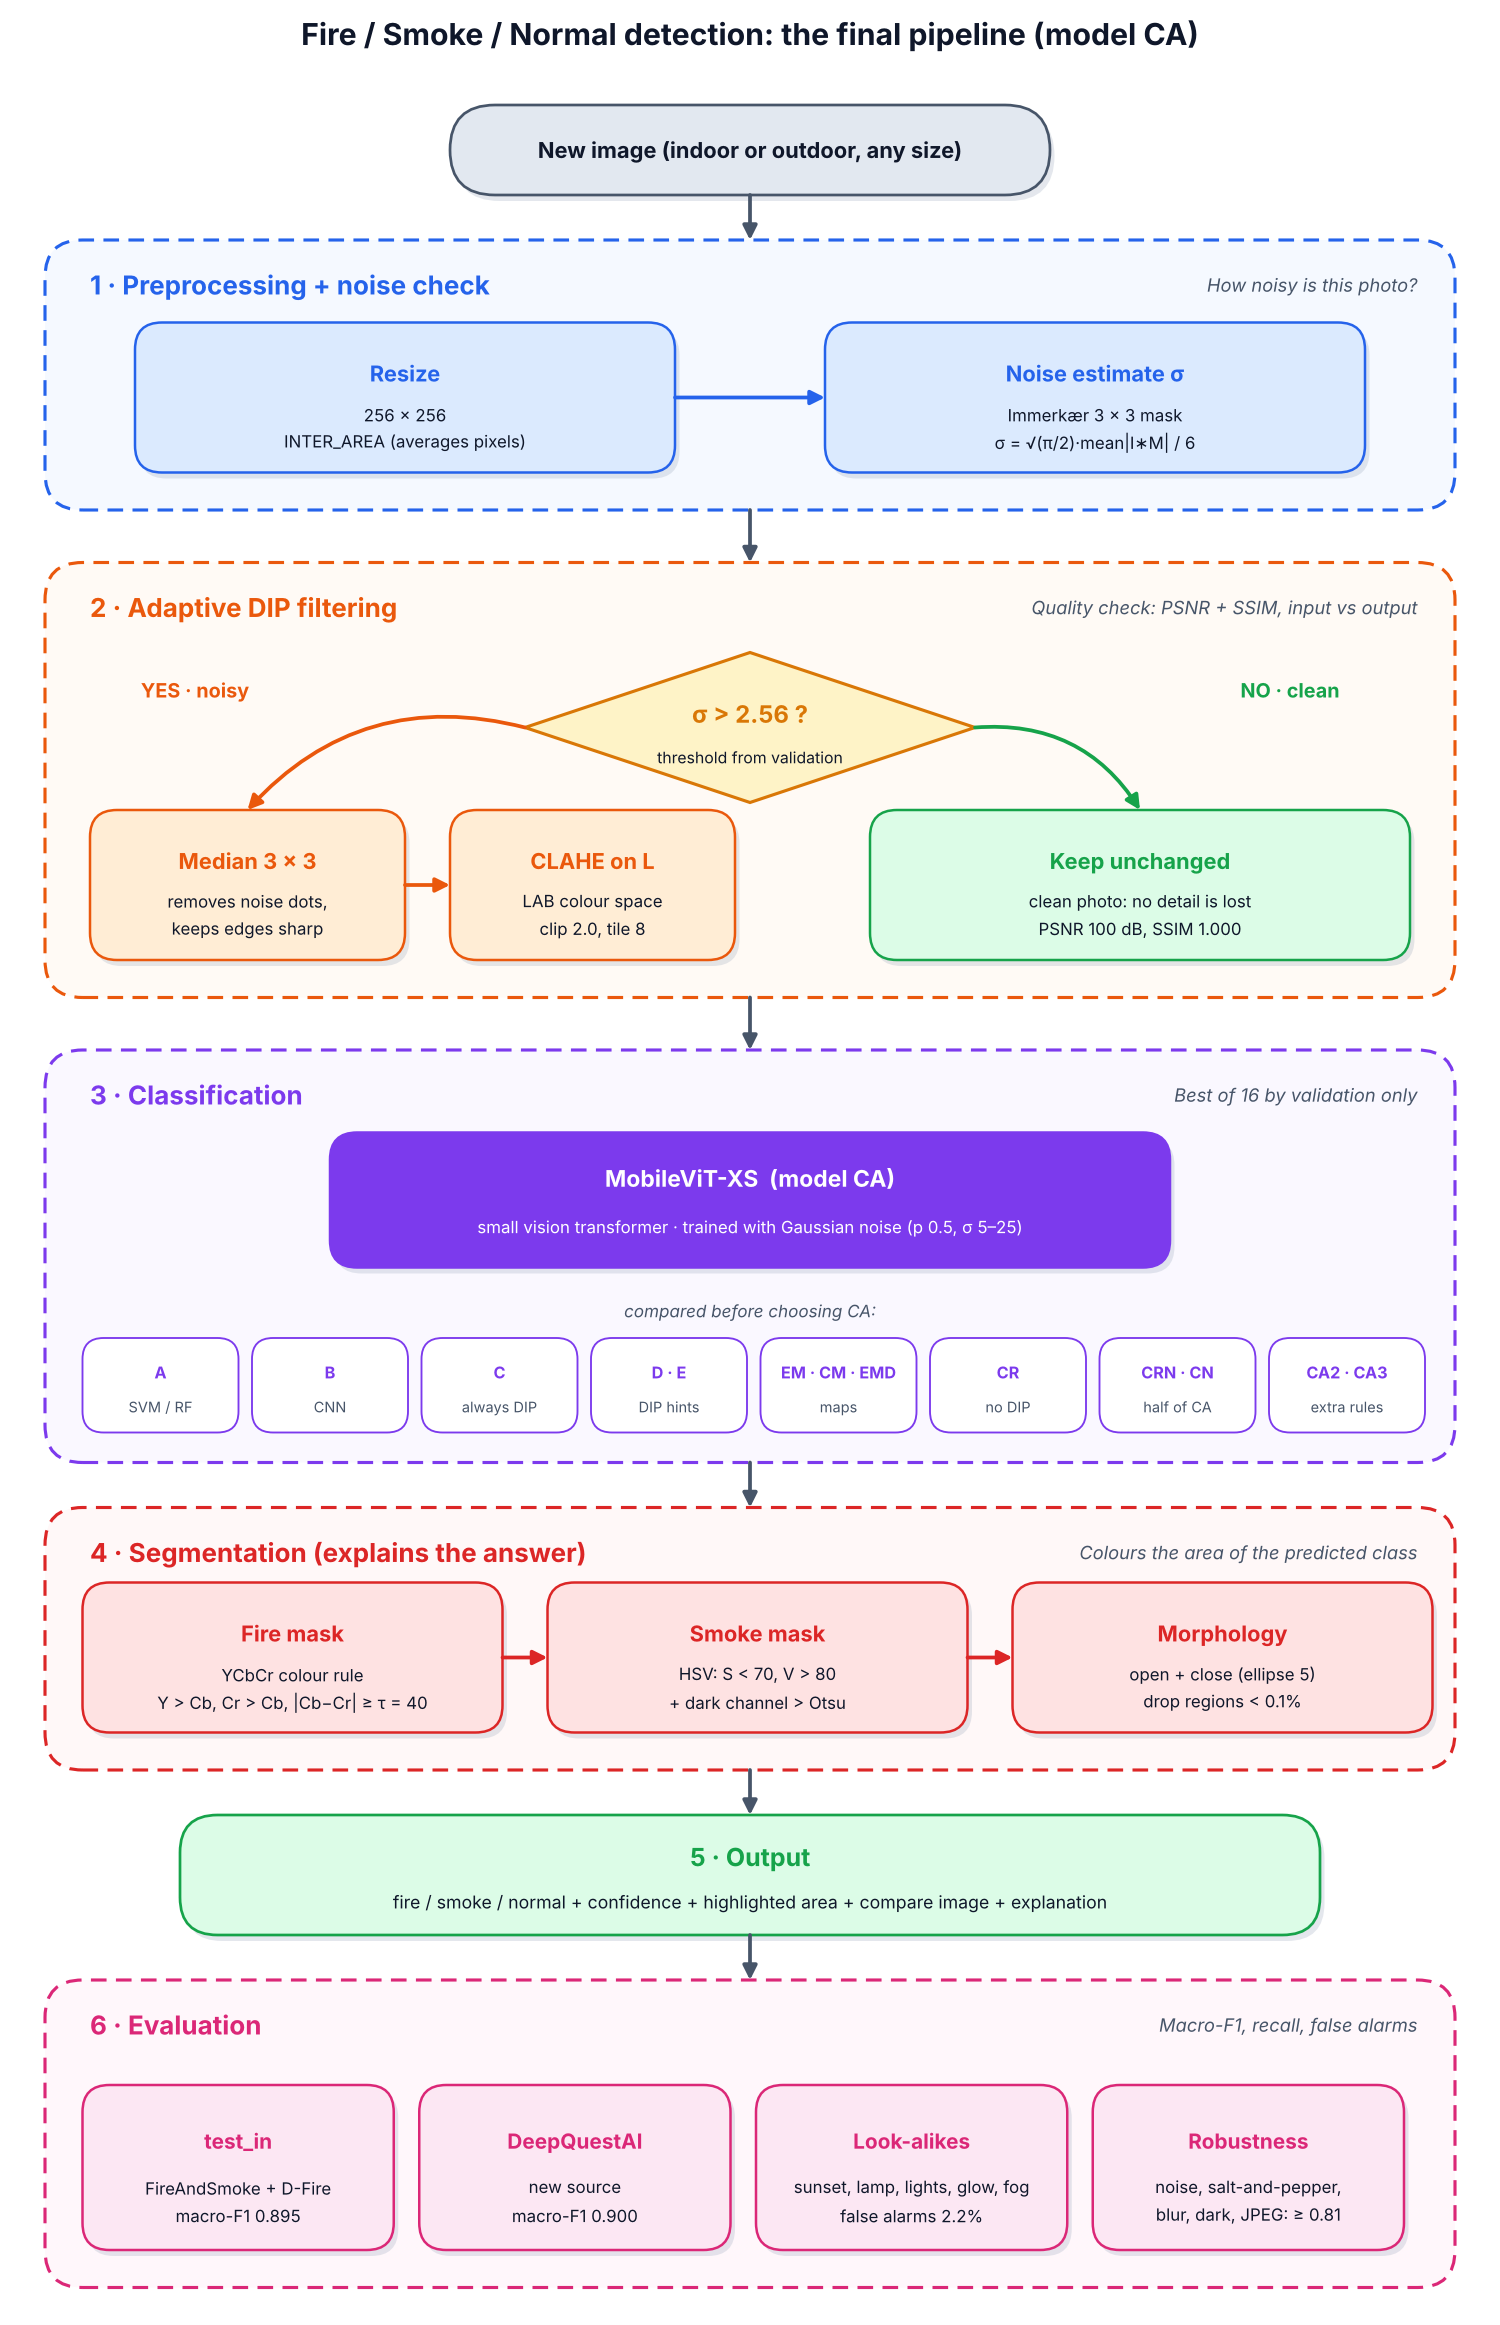
\includegraphics[width=3.48in]{fig01_pipeline.png}
  \caption{The final pipeline (model CA). A photo is filtered only when its measured noise $\sigma$ is above 2.56. The colour masks are used only to explain the answer.}
  \label{fig:pipeline}
\end{figure*}


\section{Related Work}
\subsection{Colour rules for fire}
Early fire detection methods used colour rules. Chen et al. \cite{chen} used rules on the red, green and blue values and on saturation. Töreyin et al. \cite{toreyin} added motion and flicker cues for video. Çelik and Demirel \cite{celik} gave a rule in the YCbCr colour space, which separates brightness from colour. We use their rule for our fire mask. Colour rules are fast and easy to explain, but they give false alarms on anything red or bright.

\subsection{Deep learning for fire and smoke}
Later work used convolutional neural networks (CNNs). Muhammad et al. \cite{muhammad} used a CNN for early fire detection in surveillance cameras. De Venâncio et al. \cite{dfire} built the D-Fire dataset and a detector for low-power devices. Catargiu et al. \cite{catargiu} built the FireAndSmoke dataset and compared YOLO detectors on it. That dataset also has hard normal photos that can be mistaken for fire. Small networks such as MobileNetV3 \cite{mobilenetv3} and MobileViT \cite{mobilevit} can run on small devices.

\subsection{Image quality and deep networks}
Dodge and Karam \cite{dodge} showed that noise and blur reduce the accuracy of deep networks. Hendrycks and Dietterich \cite{hendrycks} made a standard test with many kinds of image damage. Our robustness test follows the same idea. Our work joins the two lines: classic DIP is used to clean the photo, and a small transformer is used to classify it.


\section{Dataset}
\subsection{Sources}
We used three public datasets. Table \ref{tab:sources} lists them. FireAndSmoke \cite{catargiu} and D-Fire \cite{dfire} were used for training, validation and in-domain testing. Both have boxes drawn around fire and smoke. A photo with a fire box is labelled fire. A photo with only smoke boxes is labelled smoke. A photo with no box is labelled normal. The DeepQuestAI dataset \cite{deepquest} was kept only for testing. It comes from a different source, so it shows how the model works on new places and cameras.

\begin{table}[H]
  \caption{Datasets used}
  \label{tab:sources}
  \centering\footnotesize\renewcommand{\arraystretch}{1.15}
  \begin{tabular}{>{\raggedright\arraybackslash}p{1.170in}>{\raggedright\arraybackslash}p{0.780in}>{\centering\arraybackslash}p{1.300in}}
    \hline
    \textbf{Dataset} & \textbf{Photos scanned} & \textbf{Use} \\ \hline
    FireAndSmoke \cite{catargiu} & 27,294 & train, validation, test \\
    D-Fire \cite{dfire} & 21,527 & train, validation, test, mask check \\
    DeepQuestAI \cite{deepquest} & 3,000 & test only (new source) \\
    \hline
  \end{tabular}
\end{table}

\subsection{Cleaning}
The same photo often appears more than once on the internet. If a copy of a test photo is in the training set, the test score becomes too high. We removed 157 exact copies with a file hash and 9,875 near-copies with a perceptual hash (distance of 4 or less). We also removed 8,119 training and validation photos that were copies of a test photo. Fig. \ref{fig:dups} shows examples. The final dataset has 41,789 photos.

\begin{figure}[H]
  \centering
  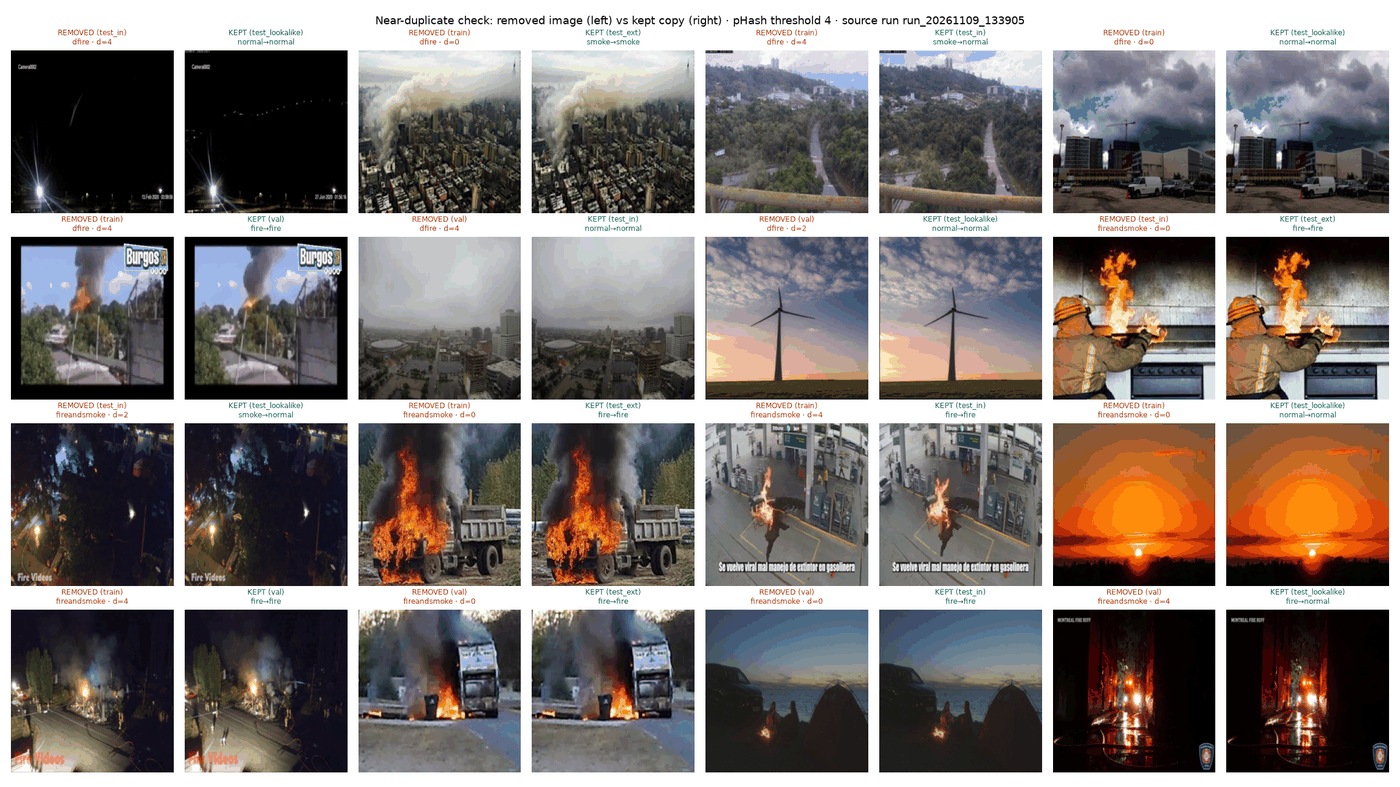
\includegraphics[width=3.50in]{fig02_dups.png}
  \caption{Examples of near-copy pairs found by the duplicate check. One photo of each pair was removed.}
  \label{fig:dups}
\end{figure}

\subsection{Splits}
Table \ref{tab:splits} shows the splits. The validation set was used to choose thresholds and the best model. The test sets were never used for any choice.

\begin{table}[H]
  \caption{Photos per split after cleaning}
  \label{tab:splits}
  \centering\footnotesize\renewcommand{\arraystretch}{1.15}
  \begin{tabular}{>{\raggedright\arraybackslash}p{0.987in}>{\centering\arraybackslash}p{0.493in}>{\centering\arraybackslash}p{0.524in}>{\centering\arraybackslash}p{0.524in}>{\centering\arraybackslash}p{0.555in}}
    \hline
    \textbf{Split} & \textbf{Fire} & \textbf{Smoke} & \textbf{Normal} & \textbf{Total} \\ \hline
    Train & 12,837 & 6,239 & 4,971 & 24,047 \\
    Validation & 4,805 & 1,922 & 598 & 7,325 \\
    Test in-domain & 2,858 & 1,930 & 2,022 & 6,810 \\
    Test DeepQuestAI & 940 & 993 & 998 & 2,931 \\
    Look-alike pool & 0 & 0 & 676 & 676 \\
    \hline
  \end{tabular}
\end{table}

\subsection{Look-alike set}
We made a separate set of normal photos that look like fire or smoke. The pool had 676 photos. We checked them by hand in a small labelling tool. We kept 451 photos in five types: sunset or sunrise (88), lamp or street light (52), vehicle light (185), reflection or glow (51) and cloud, fog or haze (75). We rejected 19 photos that really showed fire or smoke. The other photos were skipped or left unlabelled and were not used. Fig. \ref{fig:lookalike} shows one example row per type. A good model must call all of these photos normal.

\begin{figure}[H]
  \centering
  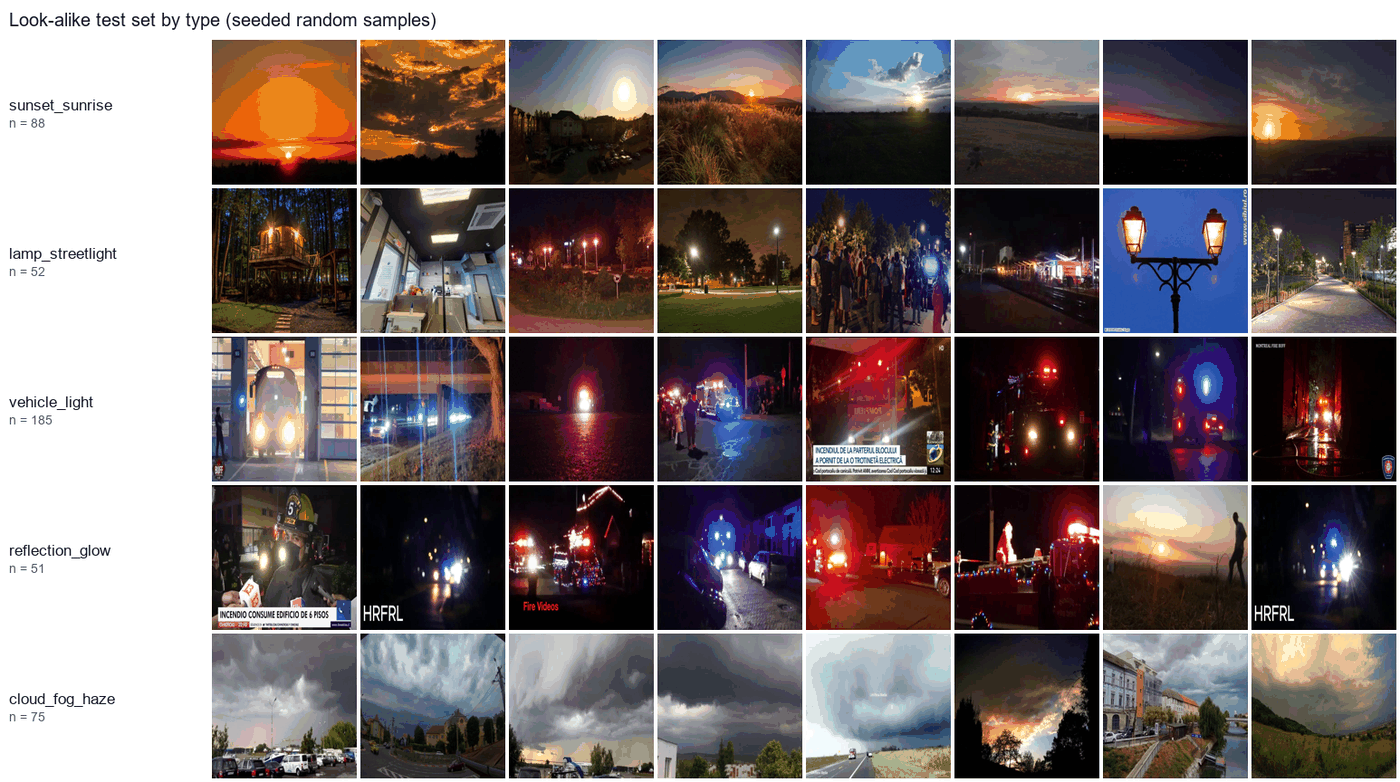
\includegraphics[width=3.50in]{fig03_lookalike.png}
  \caption{Examples of each look-alike type. A good model must call all of these normal.}
  \label{fig:lookalike}
\end{figure}


\section{Method}
\subsection{Overview}
Fig. \ref{fig:pipeline} shows the pipeline. It has four parts: resizing, noise measurement, adaptive filtering and classification. A fifth part, colour segmentation, is used only to show the user where the fire or smoke is.

\subsection{Resizing}
Each photo is resized to 256 $\times$ 256 pixels with area interpolation. Area interpolation averages blocks of pixels. It works like a low-pass filter, so it also removes a little noise \cite{gonzalez}.

\subsection{Noise measurement}
We measure the noise with the method of Immerkær \cite{immerkaer}. The grey image I is convolved with the 3 $\times$ 3 mask M:

\begin{equation}
  M=\begin{bmatrix}1&-2&1\\-2&4&-2\\1&-2&1\end{bmatrix}
\end{equation}

The mask is the difference of two Laplacian masks. Its response is zero on flat areas and on straight edges. So what is left is mostly noise. The noise level $\sigma$ is then

\begin{equation}
  \sigma=\sqrt{\frac{\pi}{2}}\;\frac{1}{6\,(W-2)(H-2)}\sum_{x,y}\left|\,(I*M)(x,y)\,\right|
\end{equation}

Here W and H are the width and height of the image. The method needs only one convolution, so it is very fast.

\subsection{Adaptive filtering}
If $\sigma$ is above 2.56, the photo is called noisy. A noisy photo gets two steps. First, a 3 $\times$ 3 median filter replaces each pixel with the middle value of its neighbours \cite{huang}. A single wrong dot is never the middle value, so it is removed, and edges stay sharp. Second, CLAHE \cite{clahe} is applied to the L channel of the LAB colour space with a clip limit of 2.0 and 8 $\times$ 8 tiles. CLAHE improves local contrast. Working on L only keeps the colours unchanged. If $\sigma$ is 2.56 or below, the photo is passed on unchanged. The threshold 2.56 was chosen on validation photos (Section V-E).

\subsection{Classifier and training}
The classifier is MobileViT-XS \cite{mobilevit} from the timm library \cite{timm}, pretrained on ImageNet. It has 1.93 million parameters. We trained it in PyTorch \cite{pytorch} for 15 epochs with the AdamW optimiser \cite{adamw}. Table \ref{tab:train} lists the settings. During training, half of the photos get extra Gaussian noise with a random $\sigma$ between 5 and 25. The noise is added before the adaptive step, so the model sees filtered noisy photos during training. This teaches the model to ignore the noise that the filter leaves behind. The epoch with the best validation macro-F1 is kept.

\begin{table}[H]
  \caption{Training settings}
  \label{tab:train}
  \centering\footnotesize\renewcommand{\arraystretch}{1.15}
  \begin{tabular}{>{\raggedright\arraybackslash}p{1.133in}>{\raggedright\arraybackslash}p{2.200in}}
    \hline
    \textbf{Setting} & \textbf{Value} \\ \hline
    Input size & 256 $\times$ 256 \\
    Batch size & 32 \\
    Epochs & 15 \\
    Optimiser & AdamW, weight decay 0.05 \\
    Learning rate & 0.0005, cosine schedule, 1 warm-up epoch \\
    Loss & cross-entropy, class weights, label smoothing 0.1 \\
    Noise training & Gaussian, probability 0.5, $\sigma$ from 5 to 25 \\
    Random seed & 42 \\
    Hardware & NVIDIA GeForce RTX 3050 (6 GB) laptop \\
    \hline
  \end{tabular}
\end{table}

\subsection{Segmentation for explanation}
After the model gives its answer, a colour mask shows the area of the predicted class. The fire mask uses the YCbCr rule of Çelik and Demirel \cite{celik}. A pixel is fire if Y $>$ Cb, Cr $>$ Cb and $|$Cb $-$ Cr$|$ $\geq$ $\tau$, with $\tau$ = 40. The smoke mask marks pixels with low saturation and enough brightness (S $<$ 70 and V $>$ 80 in HSV) whose dark channel \cite{he} is above an Otsu threshold \cite{otsu}. Both masks are cleaned with morphological opening and closing with a 5 $\times$ 5 ellipse, and regions smaller than 0.1\% of the image are removed \cite{gonzalez}. The masks do not change the answer of the model.

\subsection{Hand-made features}
For the baseline models we also turned each photo into 16 numbers: 4 colour features, 3 brightness features, 4 texture features from local binary patterns \cite{ojala} and the grey-level co-occurrence matrix \cite{haralick}, 2 haze features from the dark channel and 3 edge features.

\subsection{Models compared}
We trained 16 classifiers. Model A uses only the 16 features with an SVM \cite{svm} or a Random Forest \cite{rf}. Model B is a MobileNetV3-Small CNN \cite{mobilenetv3}. All other models use MobileViT-XS. Model C always applies the median filter and CLAHE. Model D joins the 16 features to the output of the network. Model E gives the 16 features to the transformer as extra tokens. Models EM, CM and EMD add an extra branch that predicts fire and smoke maps. Model CR uses raw photos with no DIP. CRN is CR with noise training. CN is C with noise training. CA is the adaptive model. CA2 adds a brightness rule for dark photos. CA3 picks a different filter for each noise type.

\subsection{Measures}
The main score is macro-F1, the average F1 score of the three classes. We also report recall and the false alarm rate, which is the share of normal photos called fire or smoke. For CA we report 95\% confidence intervals from 1,000 bootstrap samples \cite{efron}. Image change is measured with PSNR and SSIM \cite{ssim}:

\begin{equation}
  \mathrm{PSNR}=10\log_{10}\!\left(\frac{255^{2}}{\mathrm{MSE}}\right)
\end{equation}

MSE is the mean squared difference between two images. A higher PSNR or SSIM means that the two images are more alike.


\section{DIP Experiments}
\subsection{How much each step changes a photo}
We applied each preprocessing step to 1,300 photos and compared the output with the input. Table \ref{tab:e02} shows the result. The median filter changes a photo only a little. CLAHE changes it more, because it spreads the brightness values. Entropy rose from 7.05 to 7.33 bits and RMS contrast rose from 53.8 to 56.2. Fig. \ref{fig:steps} shows each step on example photos, and Fig. \ref{fig:hist} shows the histogram before and after CLAHE.

\begin{table}[H]
  \caption{Change caused by each step (1,300 photos, output compared with input)}
  \label{tab:e02}
  \centering\footnotesize\renewcommand{\arraystretch}{1.15}
  \begin{tabular}{>{\raggedright\arraybackslash}p{1.430in}>{\centering\arraybackslash}p{0.910in}>{\centering\arraybackslash}p{0.910in}}
    \hline
    \textbf{Step} & \textbf{PSNR (dB)} & \textbf{SSIM} \\ \hline
    Median 3 $\times$ 3 & 32.32 & 0.925 \\
    CLAHE on L & 21.07 & 0.799 \\
    Both together & 20.83 & 0.786 \\
    \hline
  \end{tabular}
\end{table}

\begin{figure}[H]
  \centering
  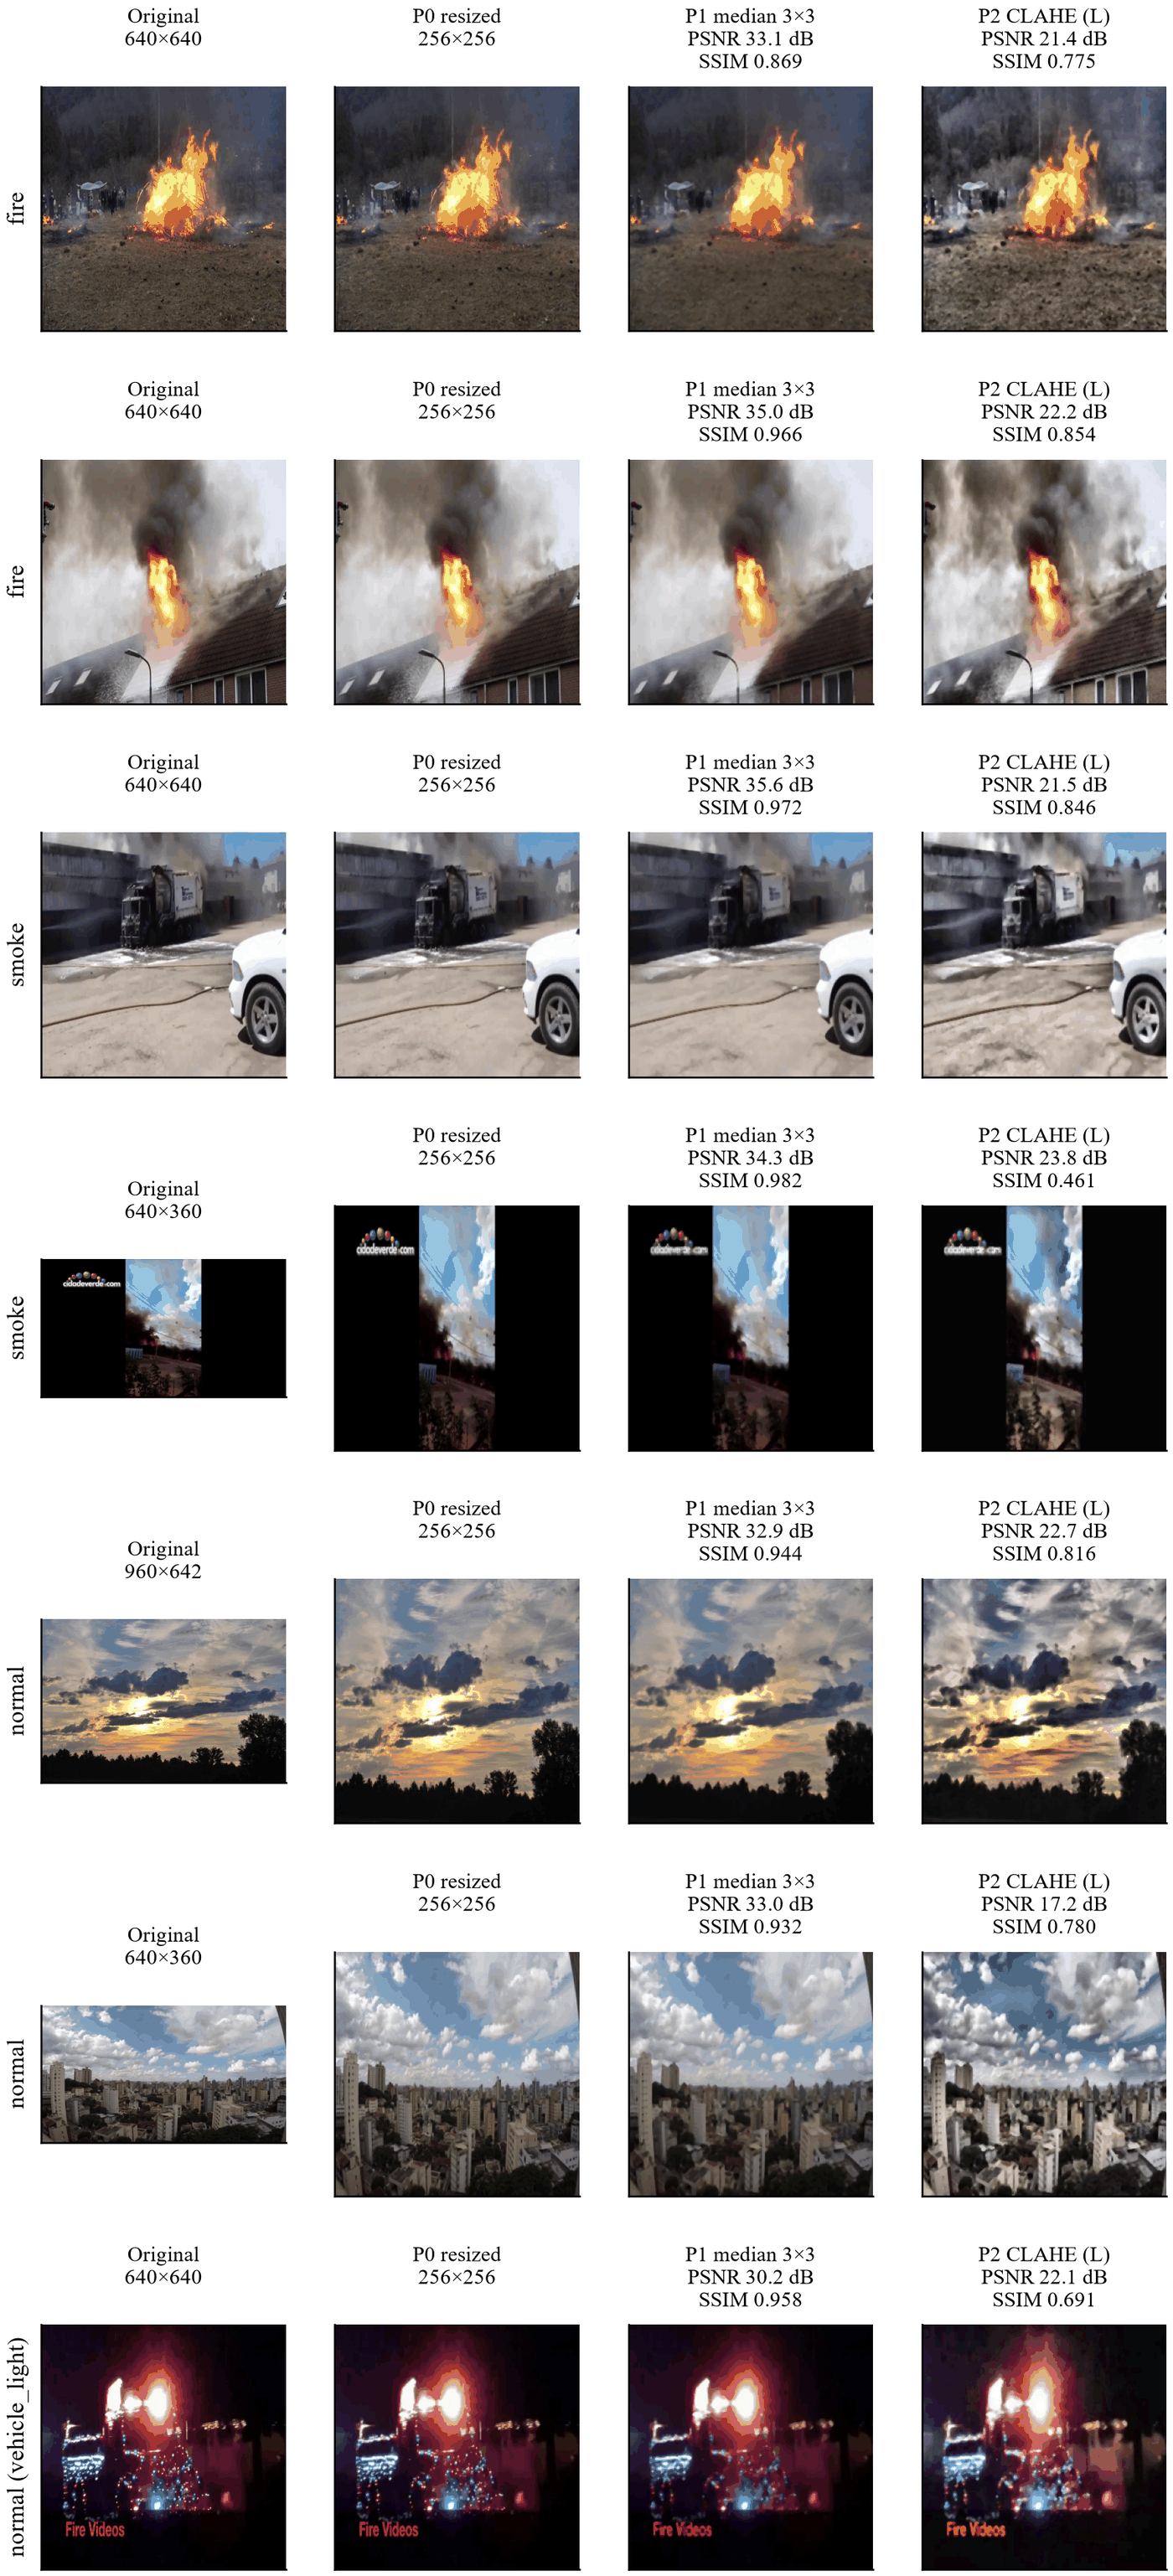
\includegraphics[width=2.46in]{fig04_steps.png}
  \caption{Each preprocessing step on example photos: original, resized, median filter, CLAHE on L.}
  \label{fig:steps}
\end{figure}

\begin{figure}[H]
  \centering
  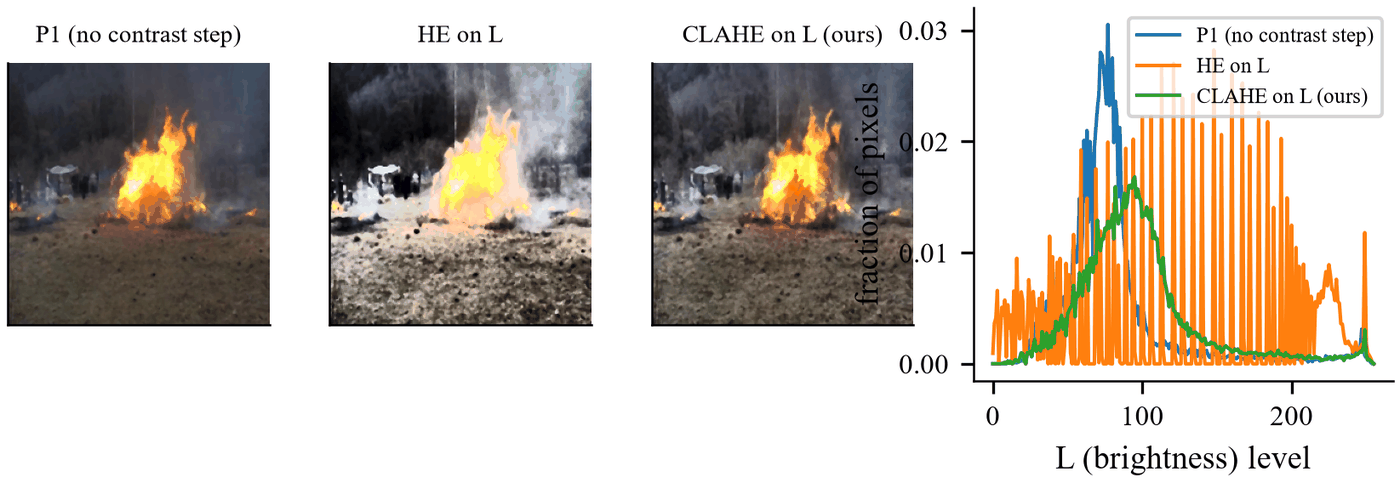
\includegraphics[width=3.50in]{fig05_hist.png}
  \caption{The brightness histogram spreads out after CLAHE.}
  \label{fig:hist}
\end{figure}

\subsection{Comparing filters and contrast methods}
We added noise to photos on purpose and tested how well each filter brings the clean photo back. Table \ref{tab:filters} shows the result. On salt-and-pepper noise the median filter is clearly the best. On Gaussian noise the bilateral filter \cite{bilateral} is the best. Fig. \ref{fig:denoise} shows an example.

\begin{table}[H]
  \caption{Restoring a noisy photo (PSNR in dB / SSIM, compared with the clean photo)}
  \label{tab:filters}
  \centering\footnotesize\renewcommand{\arraystretch}{1.15}
  \begin{tabular}{>{\raggedright\arraybackslash}p{0.887in}>{\centering\arraybackslash}p{0.760in}>{\centering\arraybackslash}p{0.760in}>{\centering\arraybackslash}p{0.760in}}
    \hline
    \textbf{Noise added} & \textbf{Median} & \textbf{Gaussian} & \textbf{Bilateral} \\ \hline
    Salt-and-pepper & 32.15 / 0.923 & 27.87 / 0.750 & 21.67 / 0.622 \\
    Gaussian & 29.97 / 0.819 & 31.10 / 0.848 & 34.56 / 0.894 \\
    \hline
  \end{tabular}
\end{table}

\begin{figure}[H]
  \centering
  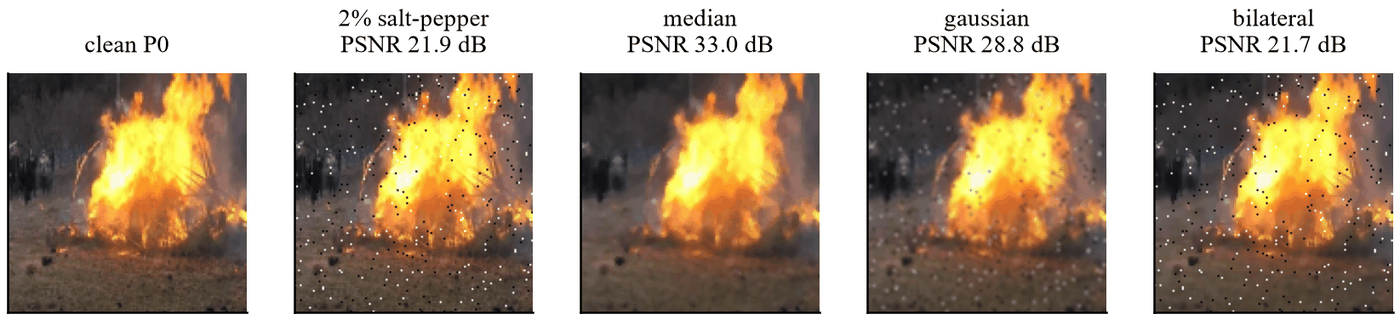
\includegraphics[width=3.50in]{fig06_denoise.png}
  \caption{Median, Gaussian and bilateral filters compared on a noisy photo.}
  \label{fig:denoise}
\end{figure}

We also compared three contrast methods by how much they shift the colours. Histogram equalisation on the RGB channels shifted colours by 18.4. Histogram equalisation on L shifted them by 1.28. CLAHE on L shifted them by only 0.32. Colour is the strongest sign of fire, so we chose CLAHE on L. Fig. \ref{fig:contrast} shows the difference.

\begin{figure}[H]
  \centering
  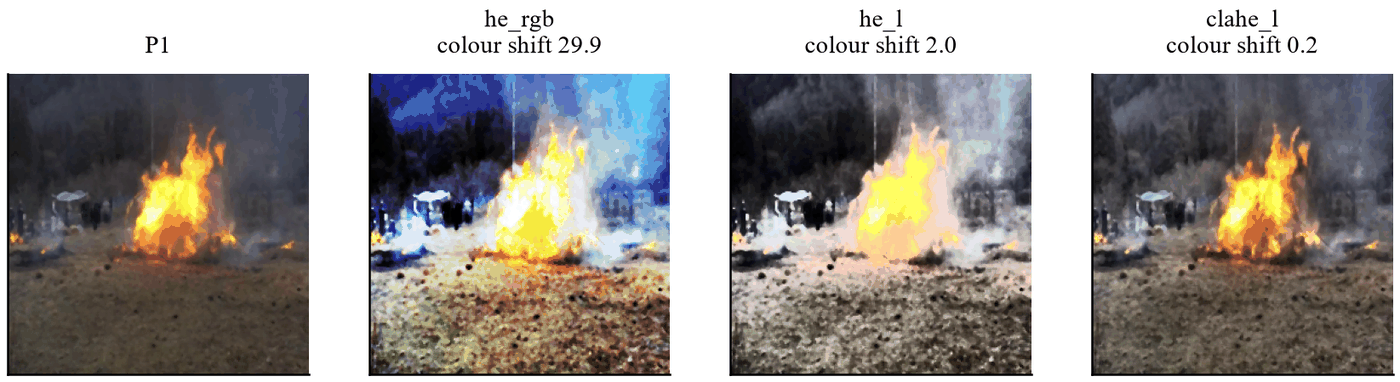
\includegraphics[width=3.50in]{fig07_contrast.png}
  \caption{Histogram equalisation on RGB changes colours a lot. CLAHE on L keeps the fire colour correct.}
  \label{fig:contrast}
\end{figure}

\subsection{Segmentation}
We checked the colour masks against the boxes of the datasets. Fig. \ref{fig:seg} shows the steps and Fig. \ref{fig:masks} shows more examples. We tested five values of the fire threshold $\tau$ on validation photos. The value $\tau$ = 40 was the best (Fig. \ref{fig:tau}). Table \ref{tab:masks} gives the result. The fire mask works fairly well. The smoke mask is weak. It marks almost 19\% of the area of normal photos, because grey sky, roads and walls have the same colour as smoke. For this reason the masks are used only as features for the baseline models and as a picture for the user.

\begin{figure}[H]
  \centering
  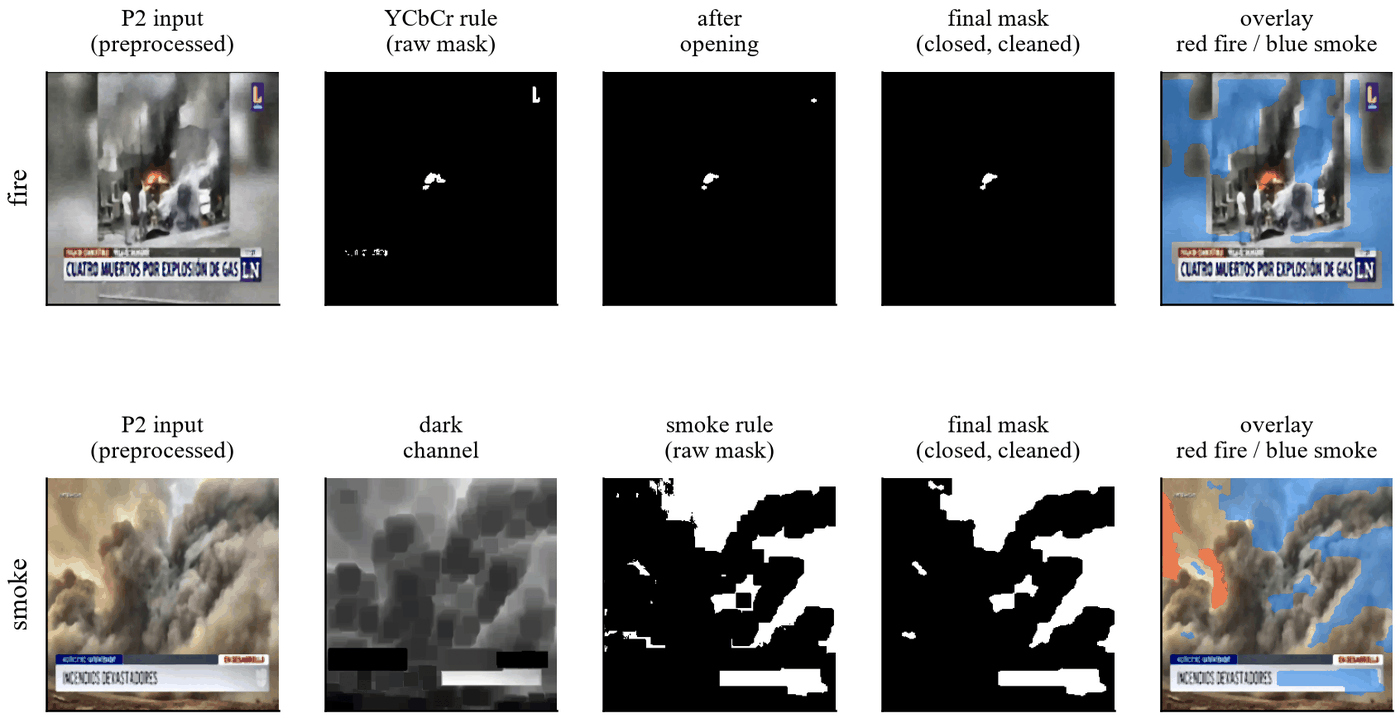
\includegraphics[width=3.50in]{fig08_seg.png}
  \caption{Segmentation step by step. Top: fire (YCbCr rule, opening, closing, overlay). Bottom: smoke (dark channel, smoke rule, cleaned mask, overlay).}
  \label{fig:seg}
\end{figure}

\begin{table}[H]
  \caption{Colour masks checked on validation photos}
  \label{tab:masks}
  \centering\footnotesize\renewcommand{\arraystretch}{1.15}
  \begin{tabular}{>{\raggedright\arraybackslash}p{0.760in}>{\centering\arraybackslash}p{0.760in}>{\centering\arraybackslash}p{1.013in}>{\centering\arraybackslash}p{0.633in}}
    \hline
    \textbf{Mask} & \textbf{Covers box area} & \textbf{Area marked on normal photos} & \textbf{Score J} \\ \hline
    Fire ($\tau$ = 40) & 33\% & 3.65\% & 0.294 \\
    Smoke & 33.7\% & 18.9\% & 0.147 \\
    \hline
  \end{tabular}
\end{table}

\begin{figure}[H]
  \centering
  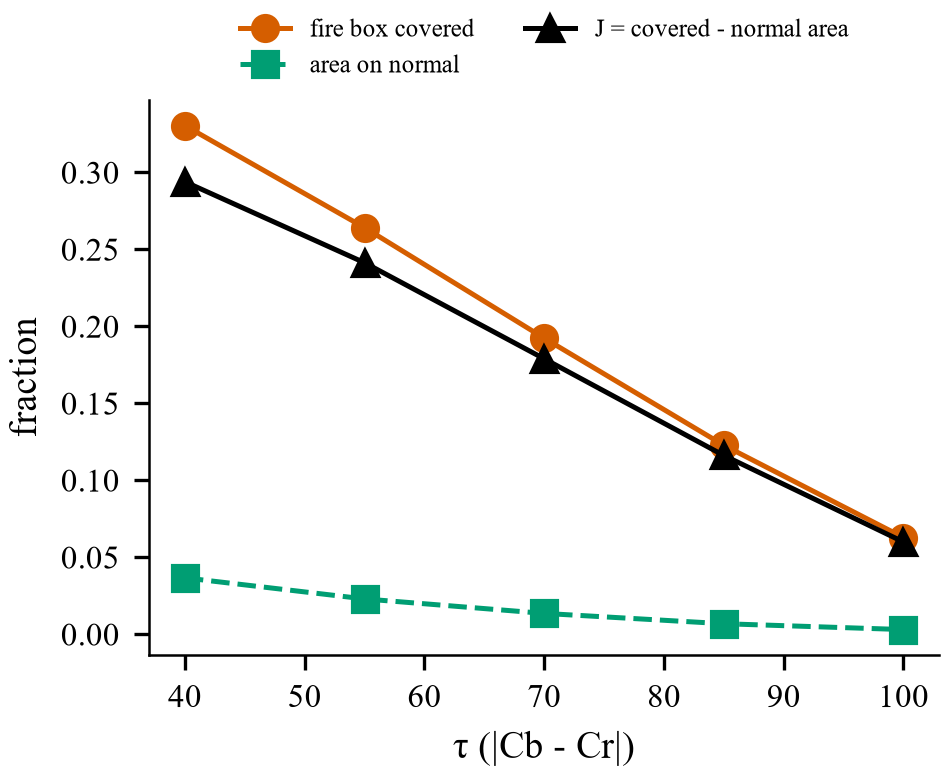
\includegraphics[width=3.50in]{fig09_tau.png}
  \caption{Choosing the fire threshold $\tau$ on validation photos. $\tau$ = 40 was the best.}
  \label{fig:tau}
\end{figure}

\begin{figure}[H]
  \centering
  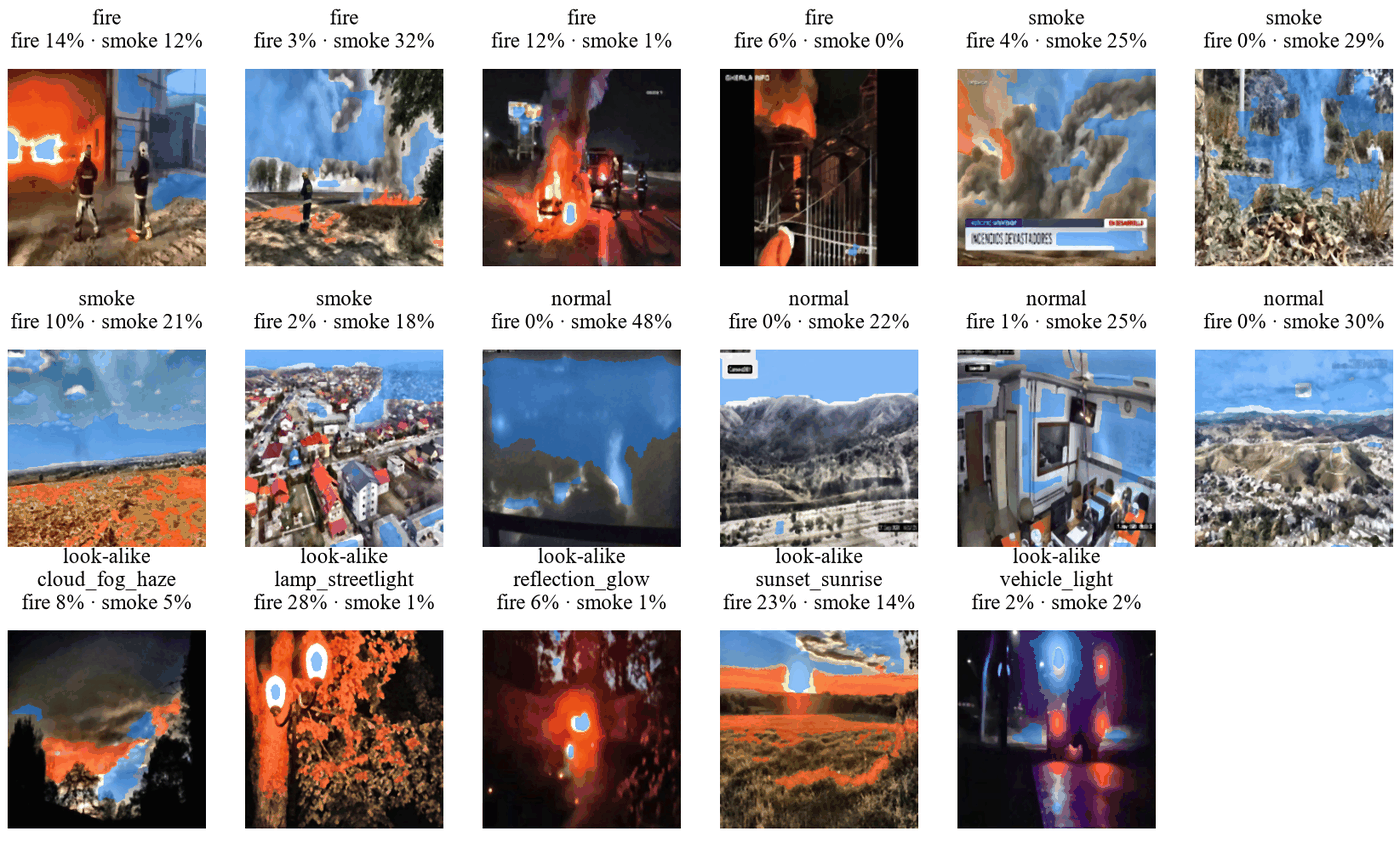
\includegraphics[width=3.50in]{fig10_masks.png}
  \caption{More mask examples. The smoke mask often also marks grey sky, roads and walls.}
  \label{fig:masks}
\end{figure}

\subsection{Features}
The 16 features were computed for 41,564 photos with no failures. This took about 22 ms per photo. Fig. \ref{fig:feat} ranks the features by the ANOVA F-score on training data. The strongest features are the edges of the fire mask (2568), redness (1452), fire area (1021) and the mean of the dark channel (999).

\begin{figure}[H]
  \centering
  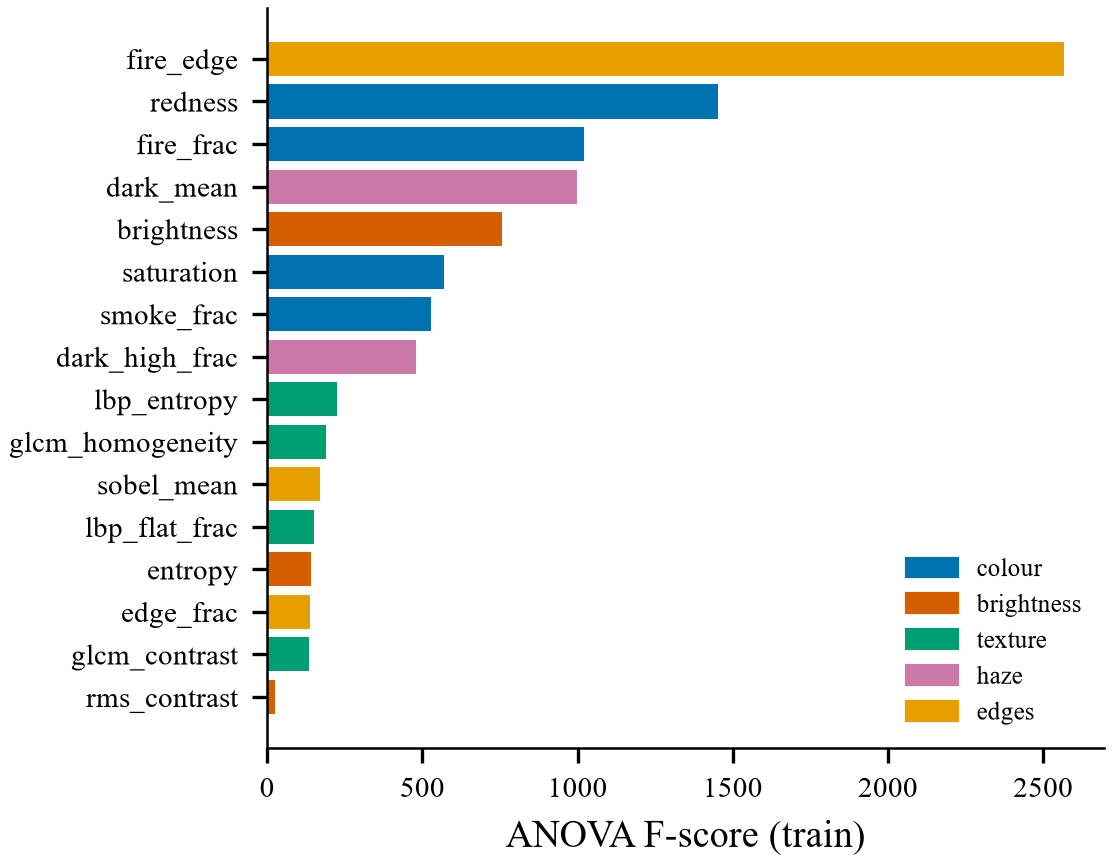
\includegraphics[width=3.50in]{fig11_feat.png}
  \caption{The 16 features ranked by ANOVA F-score on training data.}
  \label{fig:feat}
\end{figure}

\subsection{Noise threshold}
To choose the noise threshold we measured $\sigma$ on original validation photos and on the same photos with added Gaussian noise. Fig. \ref{fig:noise} shows the two groups. The threshold $\sigma$ = 2.56 separates them best, with a balanced accuracy of 0.784. It marks 97\% of the photos with added noise of $\sigma$ 15 and all photos with $\sigma$ 25. It also marks 36\% of the original photos. This is partly correct, because many camera photos already have some noise.

\begin{figure}[H]
  \centering
  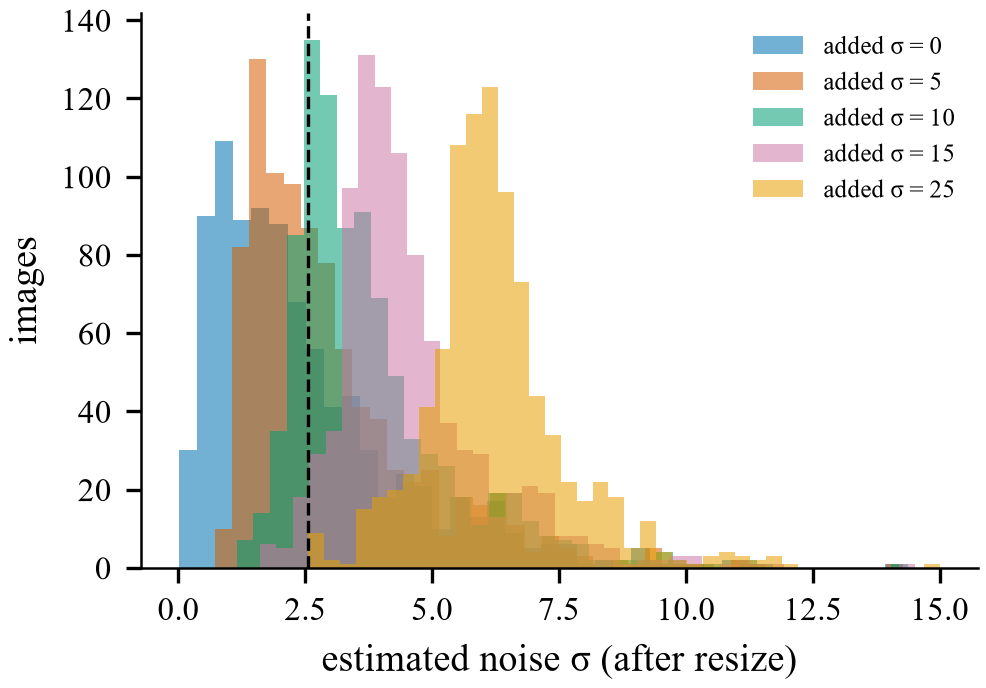
\includegraphics[width=3.50in]{fig12_noise.png}
  \caption{Noise level $\sigma$ of original photos and photos with added noise. The chosen threshold is 2.56.}
  \label{fig:noise}
\end{figure}

\subsection{Brightness threshold}
We also tested a rule for dark photos. A mean brightness of 71.4 separates normal photos from darkened photos with a balanced accuracy of 0.87 (Fig. \ref{fig:dark}). But it marks 21.9\% of ordinary photos as dark. Model CA2 used this rule. Its validation score was lower than that of CA (0.908 against 0.917), and it gave more false alarms on look-alike photos (3.1\% against 2.2\%), so the rule is not in the final model.

\begin{figure}[H]
  \centering
  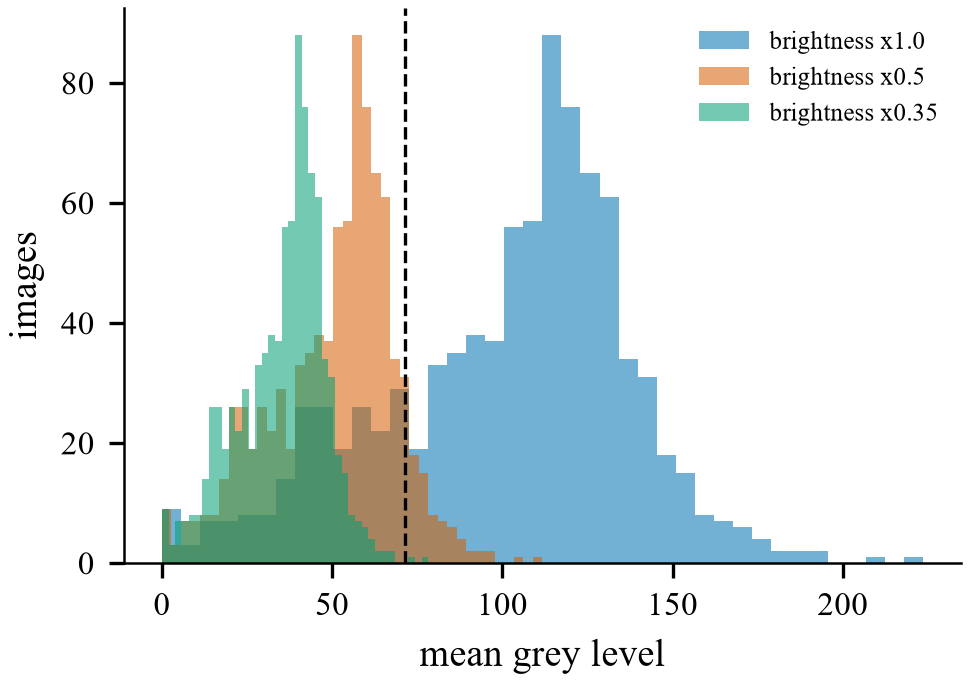
\includegraphics[width=3.50in]{fig13_dark.png}
  \caption{Mean brightness of ordinary and darkened photos. The tested threshold is 71.4.}
  \label{fig:dark}
\end{figure}

\subsection{Which filter for which noise}
In a larger study we added noise to 150 validation photos and compared 15 filter settings and a no-filter baseline. The filters included median, Gaussian, average, bilateral and non-local means \cite{nlm} filters. The first run of this study added the noise after resizing. This was a mistake, because a real camera adds noise before the photo is resized. We corrected the study and report the corrected run. Table \ref{tab:e12} shows the best filter for each noise type. Fig. \ref{fig:filtex} shows examples and Fig. \ref{fig:filtssim} shows all SSIM values.

\begin{table}[H]
  \caption{Best filter for each noise type (noise added before resizing)}
  \label{tab:e12}
  \centering\footnotesize\renewcommand{\arraystretch}{1.15}
  \begin{tabular}{>{\raggedright\arraybackslash}p{1.013in}>{\centering\arraybackslash}p{0.823in}>{\centering\arraybackslash}p{0.665in}>{\centering\arraybackslash}p{0.665in}}
    \hline
    \textbf{Noise added} & \textbf{Best filter} & \textbf{PSNR (dB)} & \textbf{SSIM} \\ \hline
    Gaussian $\sigma$ 10 & Bilateral & 37.1 & 0.932 \\
    Gaussian $\sigma$ 25 & Bilateral & 33.5 & 0.872 \\
    Salt-and-pepper 2\% & Median 3 $\times$ 3 & 31.5 & 0.903 \\
    Salt-and-pepper 5\% & Median 3 $\times$ 3 & 30.1 & 0.844 \\
    \hline
  \end{tabular}
\end{table}

\begin{figure}[H]
  \centering
  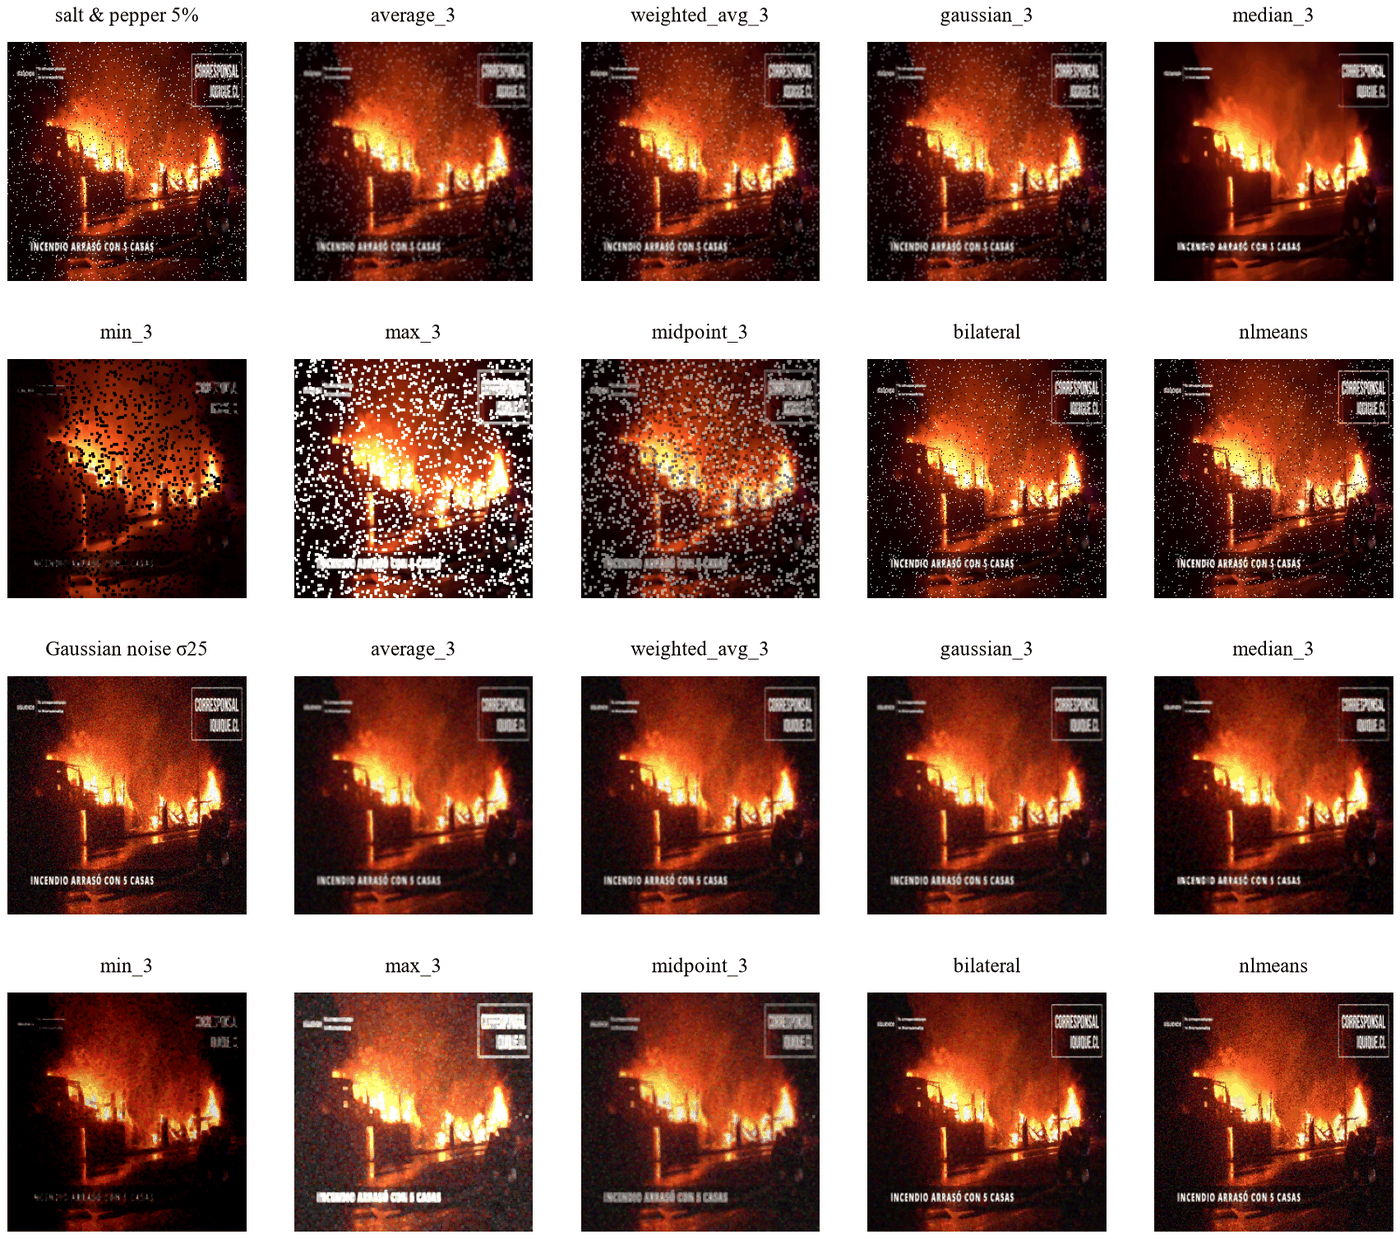
\includegraphics[width=3.50in]{fig14_filtex.png}
  \caption{The same noisy photos restored by different filters.}
  \label{fig:filtex}
\end{figure}

\begin{figure}[H]
  \centering
  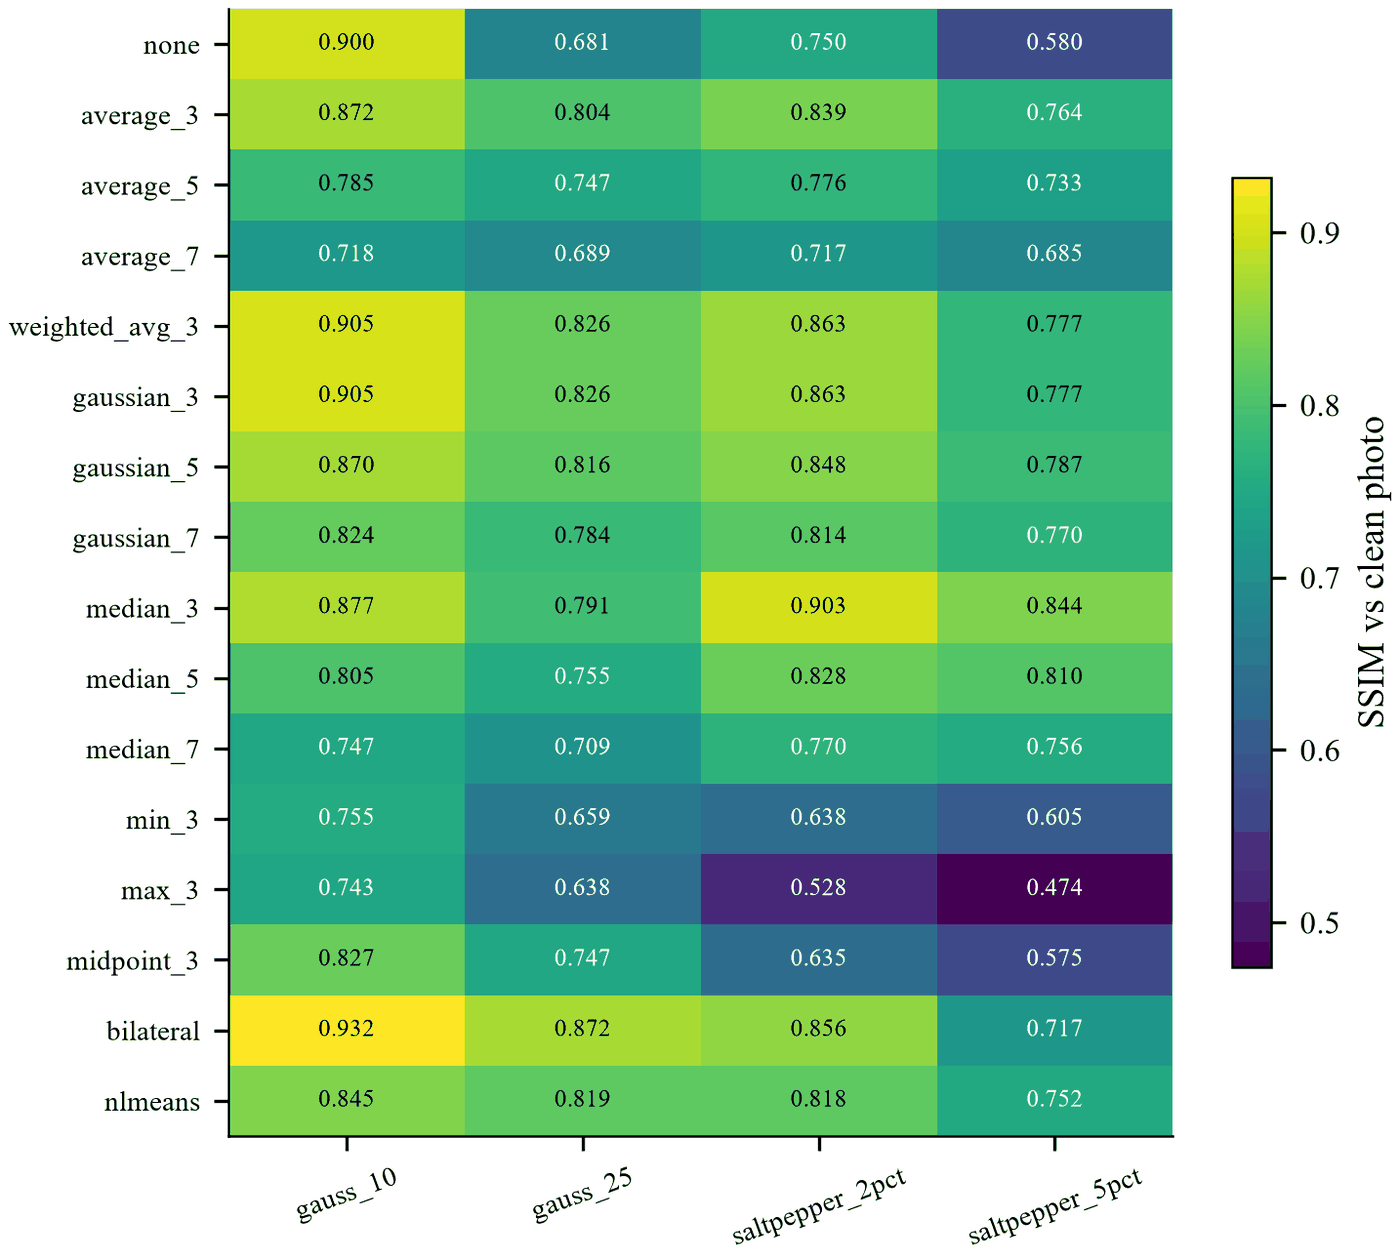
\includegraphics[width=3.50in]{fig15_filtssim.png}
  \caption{SSIM of each filter for each noise type.}
  \label{fig:filtssim}
\end{figure}

We also tested how well two detectors find noisy photos (Fig. \ref{fig:detect}). The noise estimate $\sigma$ finds both noise types, with an AUC of 0.839 for Gaussian noise and 0.964 for salt-and-pepper noise. The isolated point count (a mask with 8 in the centre and $-$1 around it, which marks lonely dots) finds salt-and-pepper noise almost perfectly when the noise is added after resizing (AUC 0.999), but poorly when it is added before (AUC 0.621). Resizing shrinks the dots into small grey spots, so they are no longer lonely points.

\begin{figure}[H]
  \centering
  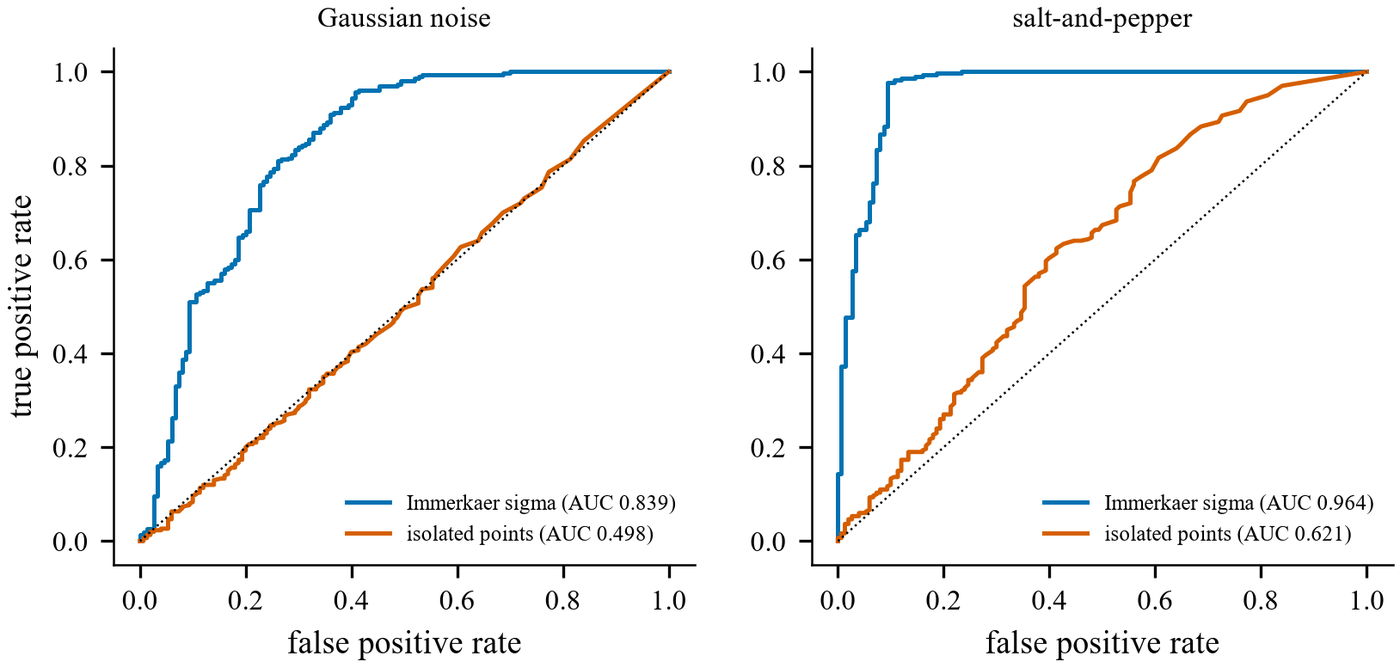
\includegraphics[width=3.50in]{fig16_detect.png}
  \caption{How well the noise estimate $\sigma$ and the isolated point count find noisy photos.}
  \label{fig:detect}
\end{figure}

Fig. \ref{fig:gallery} shows the adaptive rule on example photos. Clean photos pass unchanged, with a PSNR of 100 dB and an SSIM of 1.000. Photos with added noise are filtered.

\begin{figure}[H]
  \centering
  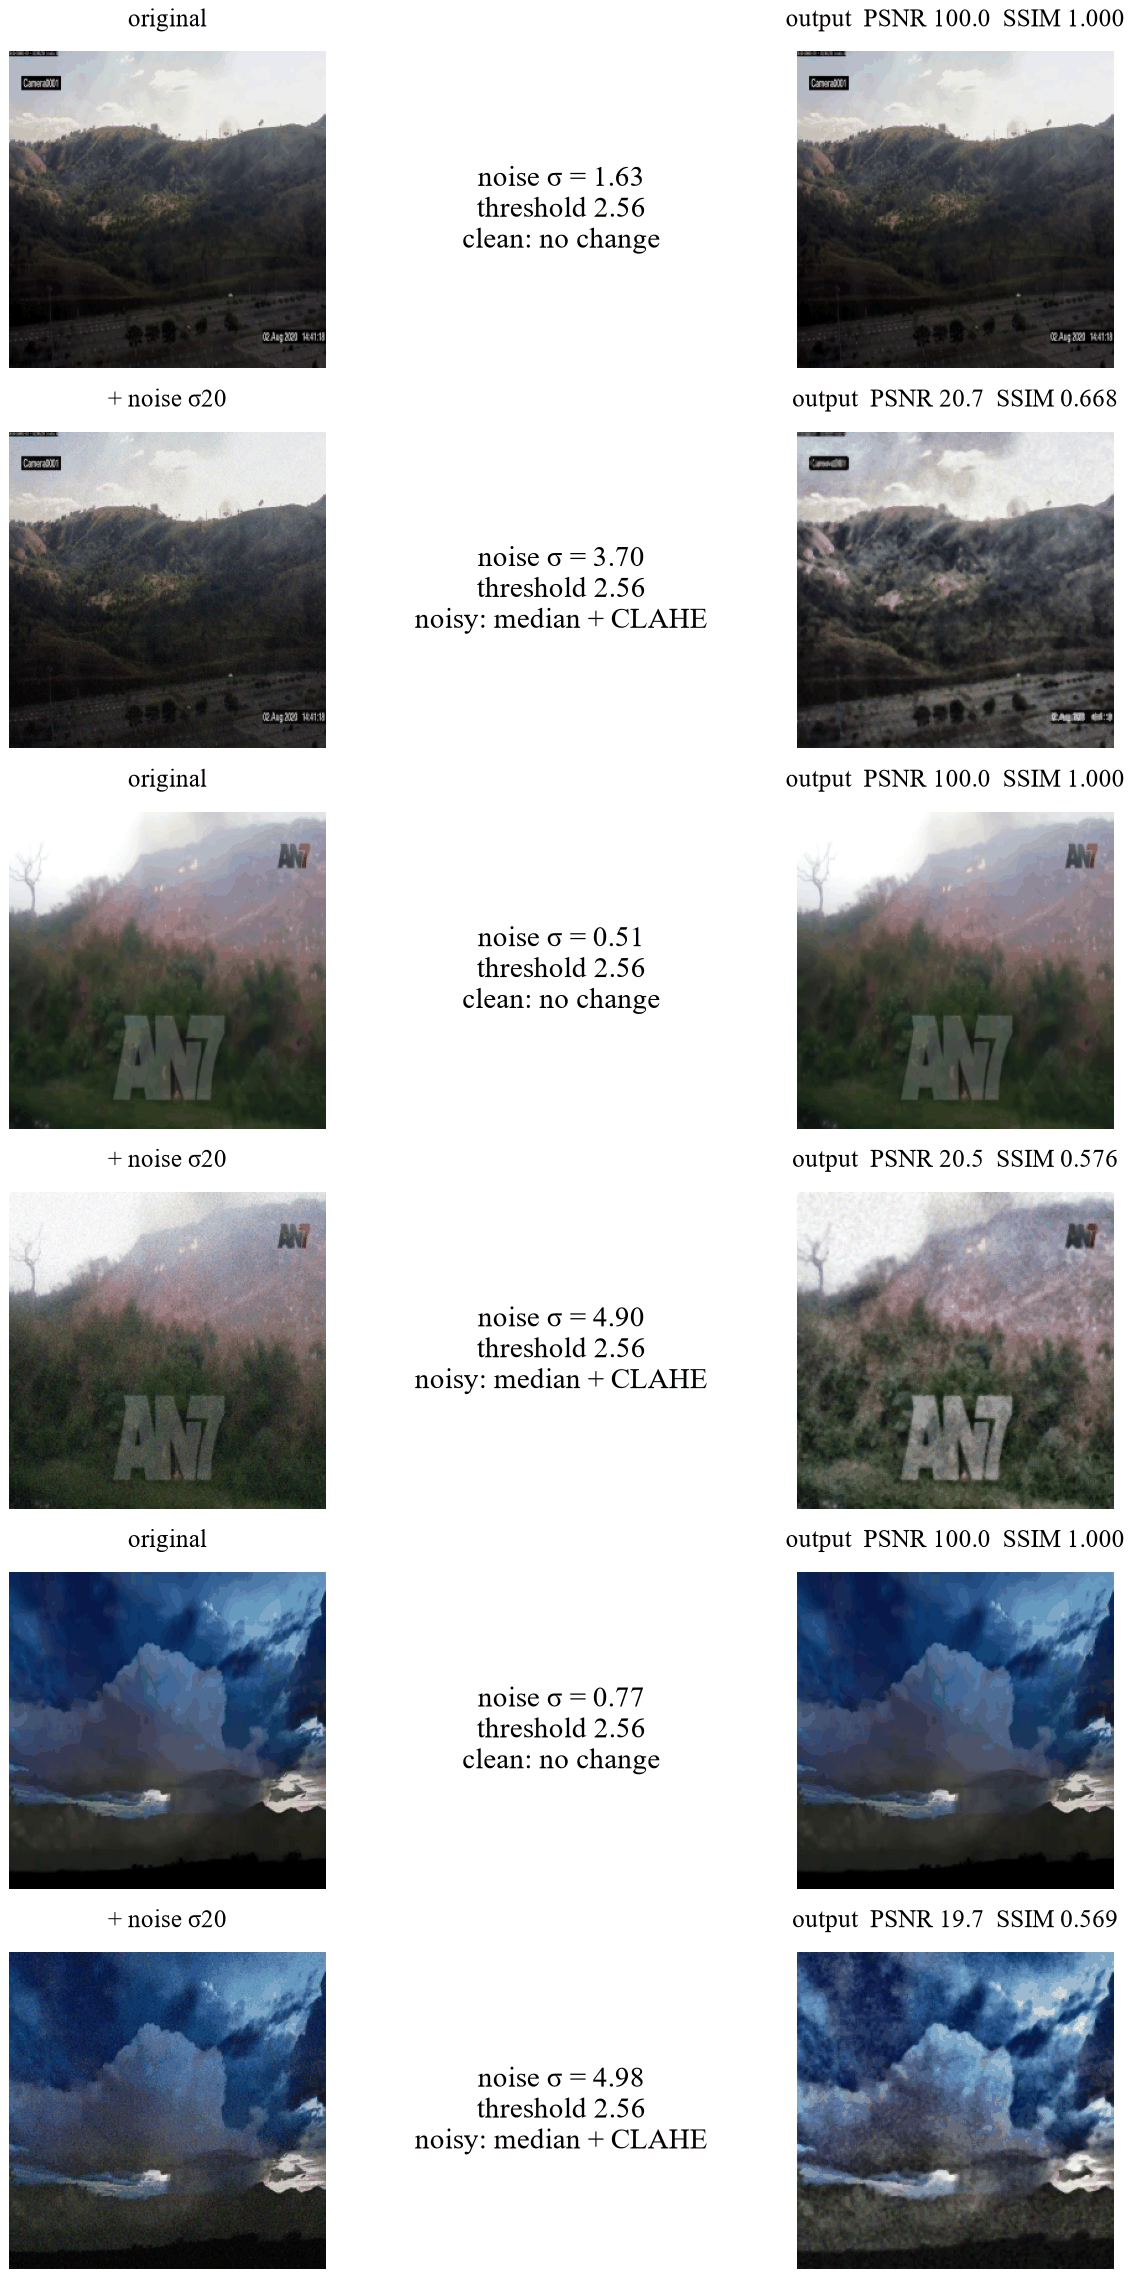
\includegraphics[width=2.69in]{fig17_gallery.png}
  \caption{The adaptive rule in action. Clean photos pass unchanged. The same photos with added noise get the median filter and CLAHE.}
  \label{fig:gallery}
\end{figure}


\section{Classification Results}
Table \ref{tab:models} gives the scores of all 16 classifiers. Fig. \ref{fig:val} shows the validation scores and Fig. \ref{fig:lachart} shows the false alarms on look-alike photos. Each model was trained once with seed 42.

\begin{table*}[!t]
  \caption{All 16 classifiers. Scores are macro-F1. False alarms are the share of normal photos called fire or smoke.}
  \label{tab:models}
  \centering\footnotesize\renewcommand{\arraystretch}{1.15}
  \begin{tabular}{>{\raggedright\arraybackslash}p{0.667in}>{\raggedright\arraybackslash}p{2.000in}>{\centering\arraybackslash}p{0.733in}>{\centering\arraybackslash}p{0.800in}>{\centering\arraybackslash}p{0.867in}>{\centering\arraybackslash}p{0.800in}>{\centering\arraybackslash}p{0.800in}}
    \hline
    \textbf{Model} & \textbf{Input and preprocessing} & \textbf{Validation} & \textbf{Test in-domain} & \textbf{Test DeepQuestAI} & \textbf{False alarms DeepQuestAI (\%)} & \textbf{False alarms look-alikes (\%)} \\ \hline
    \textbf{CA (final)} & \textbf{adaptive DIP + noise training} & \textbf{0.9174} & \textbf{0.8950} & \textbf{0.9002} & \textbf{12.4} & \textbf{2.22} \\
    CR & raw photos, no DIP & 0.9164 & 0.9017 & 0.8995 & 12.0 & 3.55 \\
    EM & feature tokens + learned maps & 0.9158 & 0.8888 & 0.8884 & 17.4 & 3.33 \\
    CA3 v2 & filter chosen per noise type (corrected) & 0.9142 & 0.8910 & 0.8912 & 15.7 & 3.55 \\
    CM & learned maps & 0.9133 & 0.8944 & 0.8753 & 16.5 & 4.21 \\
    D & 16 features joined at the end & 0.9132 & 0.8912 & 0.8981 & 10.7 & 2.66 \\
    E & 16 features as tokens & 0.9130 & 0.8945 & 0.8781 & 18.7 & 3.55 \\
    EMD & feature tokens + maps from DIP masks & 0.9102 & 0.8871 & 0.8827 & 13.1 & 2.66 \\
    CRN & raw photos + noise training & 0.9092 & 0.8905 & 0.8974 & 13.2 & 3.55 \\
    CA3 v1 & filter chosen per noise type (first run) & 0.9089 & 0.8883 & 0.9044 & 13.1 & 2.66 \\
    CA2 & adaptive DIP + brightness rule & 0.9078 & 0.8901 & 0.9010 & 10.5 & 3.10 \\
    C & always median + CLAHE & 0.9077 & 0.8897 & 0.8833 & 15.5 & 3.30 \\
    CN & always median + CLAHE + noise training & 0.8991 & 0.8868 & 0.8871 & 16.8 & 2.88 \\
    B & MobileNetV3-Small CNN & 0.8859 & 0.8776 & 0.8555 & 22.2 & 3.55 \\
    A (RF) & 16 features, Random Forest & 0.6955 & 0.7105 & 0.5078 & 81.6 & 40.8 \\
    A (SVM) & 16 features, SVM & 0.6416 & 0.6896 & 0.5243 & 76.8 & 35.7 \\
    \hline
  \end{tabular}
\end{table*}

\begin{figure}[H]
  \centering
  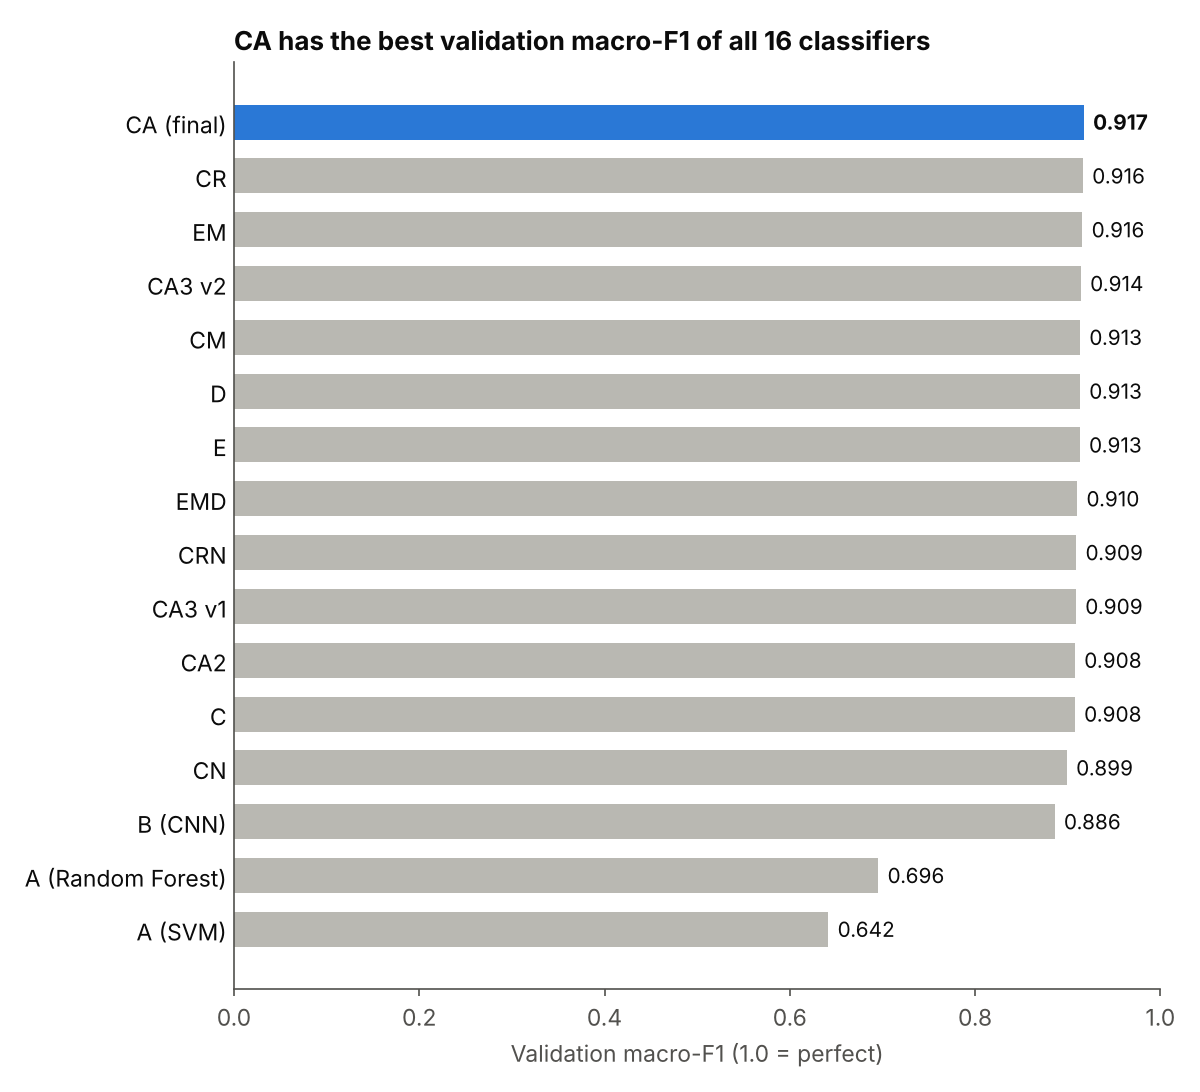
\includegraphics[width=3.50in]{fig18_val.png}
  \caption{Validation macro-F1 of all 16 classifiers. Only this score was used to choose the final model.}
  \label{fig:val}
\end{figure}

\begin{figure}[H]
  \centering
  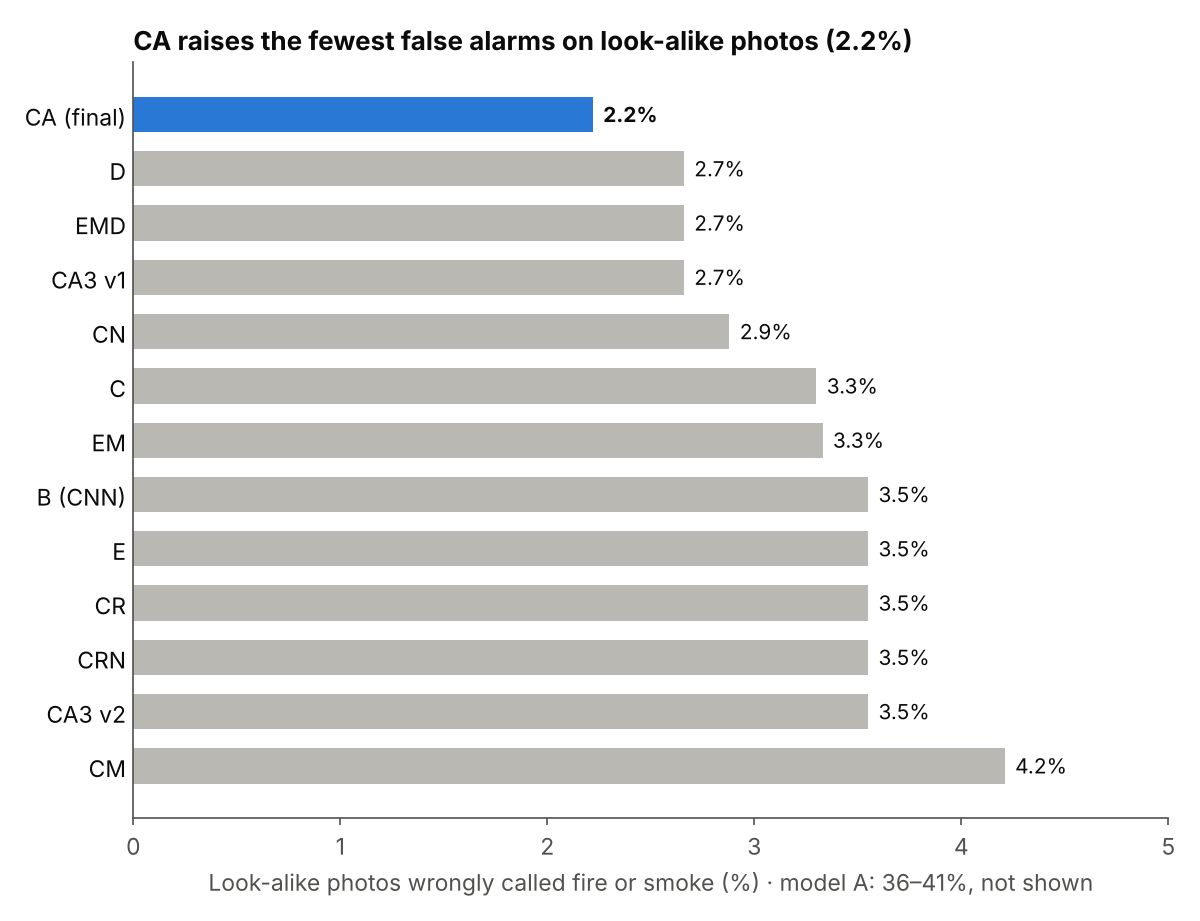
\includegraphics[width=3.50in]{fig19_lachart.png}
  \caption{Share of look-alike photos wrongly called fire or smoke. Model A (36\% to 41\%) is not shown.}
  \label{fig:lachart}
\end{figure}

\subsection{Baselines}
Model A reaches only 0.70 on validation and about 0.51 on DeepQuestAI. It calls 77\% to 82\% of the normal DeepQuestAI photos fire or smoke (Fig. \ref{fig:cma}). Sixteen numbers cannot describe a photo well enough. Model B, the CNN, reaches 0.886 on validation. Every MobileViT-XS model is better than B.

\begin{figure}[H]
  \centering
  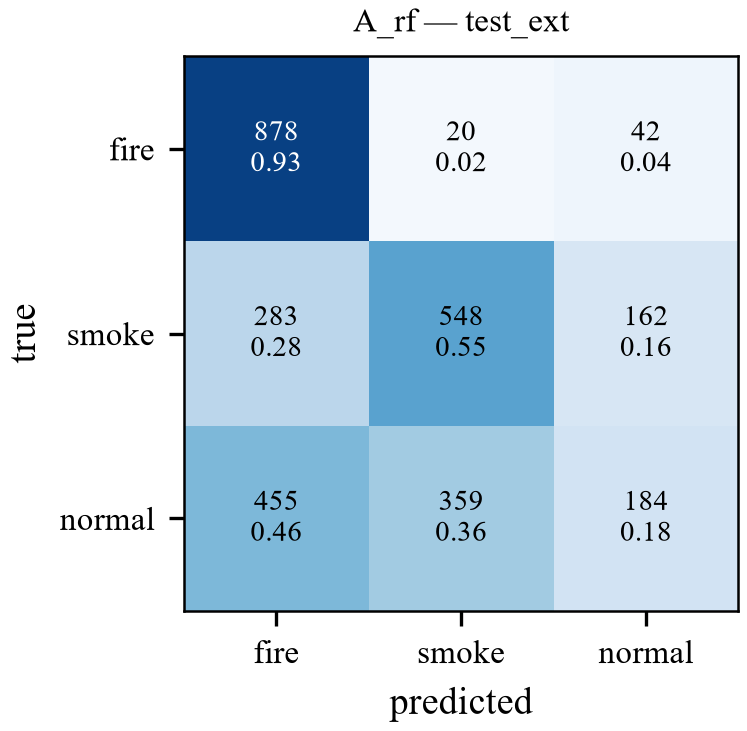
\includegraphics[width=2.60in]{fig20_cma.png}
  \caption{Confusion matrix of model A (Random Forest) on DeepQuestAI. Most normal photos are called fire or smoke.}
  \label{fig:cma}
\end{figure}

\subsection{Models with DIP features inside the network}
Models D, E, EM, CM and EMD give DIP information to the network in different ways. Fig. \ref{fig:maps} shows maps learned by model EM. Their validation scores are between 0.910 and 0.916. None of them is better than CA. To see if these models really use the features, we switched off one group of features at test time (Fig. \ref{fig:ablate}). For D and EM the macro-F1 changed by less than 0.5 points. Only model E lost a little on DeepQuestAI (0.013 for texture and 0.011 for edges). So the transformer learns almost everything from the photo itself. After this result we stopped adding features and worked on cleaning the photo instead.

\begin{figure}[H]
  \centering
  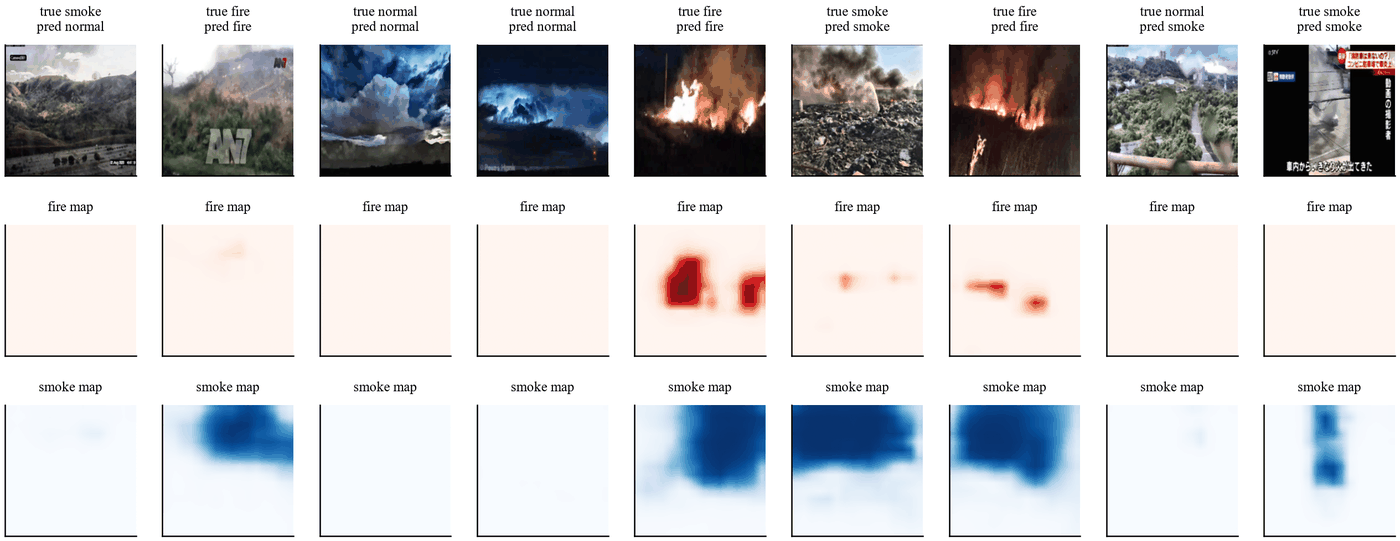
\includegraphics[width=3.50in]{fig21_maps.png}
  \caption{Fire and smoke maps learned by model EM.}
  \label{fig:maps}
\end{figure}

\begin{figure}[H]
  \centering
  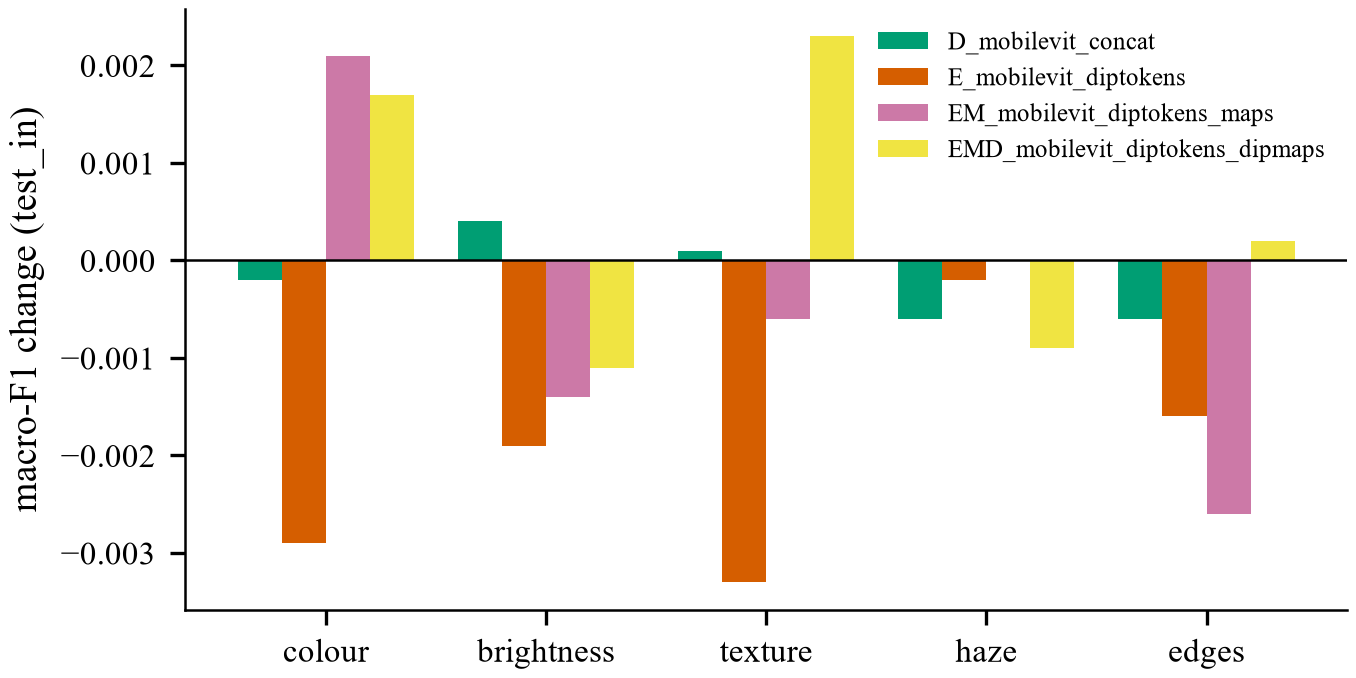
\includegraphics[width=3.50in]{fig22_ablate.png}
  \caption{Change in macro-F1 on the in-domain test set when one group of features is switched off at test time.}
  \label{fig:ablate}
\end{figure}

\subsection{Raw photos against DIP}
Model CR uses raw photos. On clean photos it is very good. It has the best in-domain test score (0.902). Model C, which filters every photo, is a little lower on all three sets. This shows that filtering clean photos does not help. But the robustness test in Section VI-E shows that CR breaks down on noisy photos.

\subsection{The final model}
Model CA has the best validation macro-F1 of all 16 classifiers (0.9174), so it was chosen as the final model. Table \ref{tab:ca} gives its scores with 95\% confidence intervals. Fig. \ref{fig:curve} shows the training curve and Fig. \ref{fig:cmca} shows the confusion matrix on DeepQuestAI. On the in-domain test set, the fire recall is 0.955 and the smoke recall is 0.815. CA is not the best on every single test. CR is higher on the in-domain test, CA3 v1 and CA2 are a little higher on DeepQuestAI, and CA2 and D have fewer false alarms on DeepQuestAI. The macro-F1 differences are small and lie inside the confidence intervals of CA.

\begin{table}[H]
  \caption{Final model CA with 95\% confidence intervals}
  \label{tab:ca}
  \centering\footnotesize\renewcommand{\arraystretch}{1.15}
  \begin{tabular}{>{\raggedright\arraybackslash}p{0.720in}>{\centering\arraybackslash}p{0.360in}>{\centering\arraybackslash}p{0.420in}>{\centering\arraybackslash}p{0.420in}>{\centering\arraybackslash}p{0.660in}>{\centering\arraybackslash}p{0.420in}}
    \hline
    \textbf{Split} & \textbf{Photos} & \textbf{Accuracy} & \textbf{Macro-F1} & \textbf{Macro-F1 95\% interval} & \textbf{False alarms} \\ \hline
    Validation & 7,325 & 0.942 & 0.917 & 0.9085 to 0.9257 & 5.5\% \\
    Test in-domain & 6,810 & 0.904 & 0.895 & 0.8877 to 0.9024 & 8.3\% \\
    Test DeepQuestAI & 2,931 & 0.900 & 0.900 & 0.8898 to 0.9116 & 12.4\% \\
    Look-alikes & 451 & n/a & n/a & n/a & 2.2\% \\
    \hline
  \end{tabular}
\end{table}

\begin{figure}[H]
  \centering
  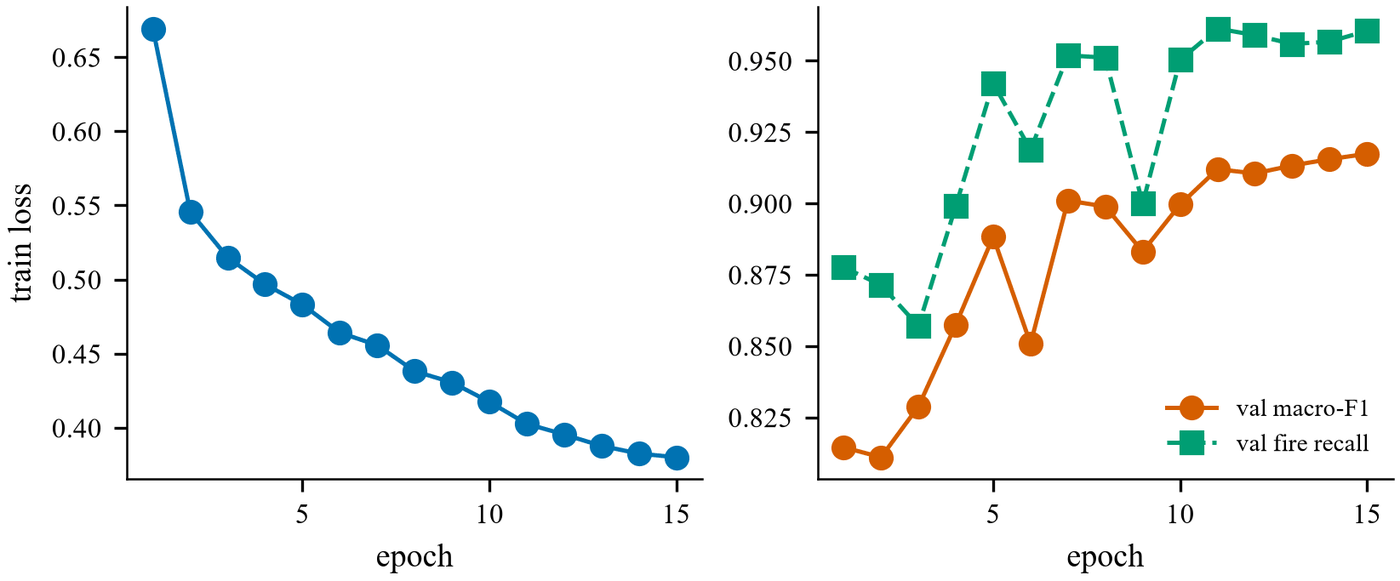
\includegraphics[width=3.50in]{fig23_curve.png}
  \caption{Training curve of model CA. The best epoch was the last one, epoch 15.}
  \label{fig:curve}
\end{figure}

\begin{figure}[H]
  \centering
  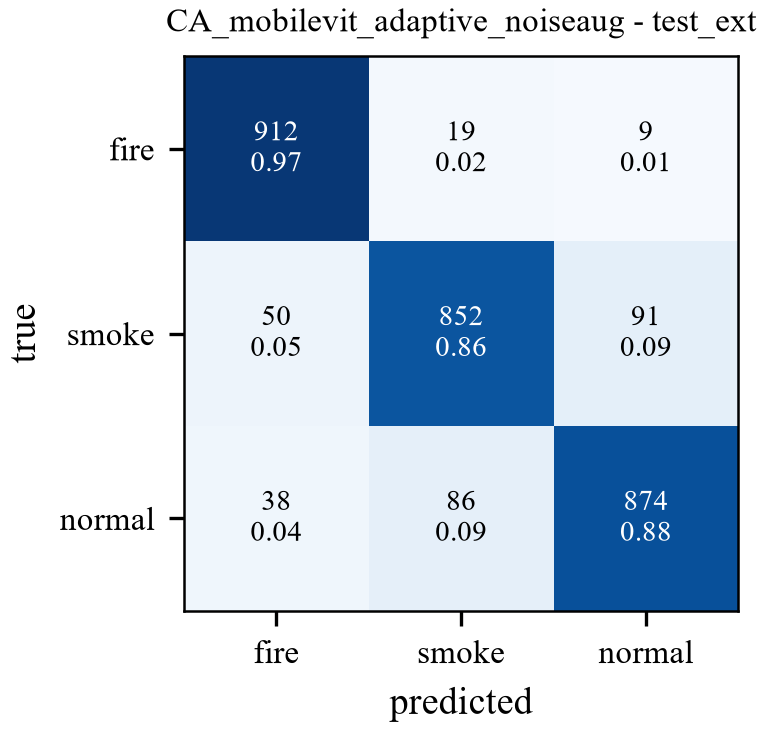
\includegraphics[width=2.60in]{fig24_cmca.png}
  \caption{Confusion matrix of model CA on DeepQuestAI.}
  \label{fig:cmca}
\end{figure}

Table \ref{tab:latypes} shows the false alarms of CA on each look-alike type. Only 10 of the 451 photos were called fire or smoke. No fog photo was called smoke.

\begin{table}[H]
  \caption{False alarms of model CA on the look-alike set}
  \label{tab:latypes}
  \centering\footnotesize\renewcommand{\arraystretch}{1.15}
  \begin{tabular}{>{\raggedright\arraybackslash}p{0.925in}>{\centering\arraybackslash}p{0.432in}>{\centering\arraybackslash}p{0.524in}>{\centering\arraybackslash}p{0.586in}>{\centering\arraybackslash}p{0.617in}}
    \hline
    \textbf{Type} & \textbf{Photos} & \textbf{Called fire} & \textbf{Called smoke} & \textbf{False alarm rate} \\ \hline
    Cloud, fog, haze & 75 & 0 & 0 & 0.00\% \\
    Lamp, street light & 52 & 2 & 0 & 3.85\% \\
    Reflection, glow & 51 & 1 & 1 & 3.92\% \\
    Sunset, sunrise & 88 & 0 & 1 & 1.14\% \\
    Vehicle light & 185 & 0 & 5 & 2.70\% \\
    All & 451 & 3 & 7 & 2.22\% \\
    \hline
  \end{tabular}
\end{table}

\subsection{Robustness to damaged photos}
We damaged the DeepQuestAI photos on purpose and measured macro-F1 again. Nothing was retrained. The damage was added to the full-size photo, before the pipeline. We used nine kinds of damage: darkening (brightness times 0.35), Gaussian blur (7 $\times$ 7 kernel), JPEG compression (quality 20), Gaussian noise with $\sigma$ of 5, 10, 15 and 25, and salt-and-pepper noise on 2\% and 5\% of the pixels. Table \ref{tab:robust} and Fig. \ref{fig:robust} show the result.

\begin{table*}[!t]
  \caption{Macro-F1 on DeepQuestAI photos with added damage (S\&P = salt-and-pepper noise)}
  \label{tab:robust}
  \centering\footnotesize\renewcommand{\arraystretch}{1.15}
  \begin{tabular}{>{\raggedright\arraybackslash}p{0.760in}>{\centering\arraybackslash}p{0.557in}>{\centering\arraybackslash}p{0.557in}>{\centering\arraybackslash}p{0.557in}>{\centering\arraybackslash}p{0.557in}>{\centering\arraybackslash}p{0.557in}>{\centering\arraybackslash}p{0.557in}>{\centering\arraybackslash}p{0.557in}>{\centering\arraybackslash}p{0.557in}>{\centering\arraybackslash}p{0.557in}>{\centering\arraybackslash}p{0.557in}}
    \hline
    \textbf{Model} & \textbf{Clean} & \textbf{Dark} & \textbf{Blur} & \textbf{JPEG} & \textbf{Noise $\sigma$ 5} & \textbf{Noise $\sigma$ 10} & \textbf{Noise $\sigma$ 15} & \textbf{Noise $\sigma$ 25} & \textbf{S\&P 2\%} & \textbf{S\&P 5\%} \\ \hline
    \textbf{CA (final)} & \textbf{0.9002} & \textbf{0.8678} & \textbf{0.8887} & \textbf{0.8772} & \textbf{0.8937} & \textbf{0.8759} & \textbf{0.8599} & \textbf{0.8145} & \textbf{0.8632} & \textbf{0.8197} \\
    CA2 & 0.9010 & 0.8772 & 0.8813 & 0.8868 & 0.8942 & 0.8843 & 0.8684 & 0.8365 & 0.8611 & 0.8187 \\
    CA3 v2 & 0.8912 & 0.8739 & 0.8809 & 0.8673 & 0.8870 & 0.8751 & 0.8560 & 0.7628 & 0.8408 & 0.7907 \\
    CN & 0.8871 & 0.8838 & 0.8678 & 0.8612 & 0.8815 & 0.8698 & 0.8569 & 0.7983 & 0.8430 & 0.7879 \\
    CRN & 0.8974 & 0.8776 & 0.8858 & 0.8859 & 0.8984 & 0.8876 & 0.8696 & 0.8058 & 0.6857 & 0.4407 \\
    CR & 0.8995 & 0.8895 & 0.9062 & 0.8731 & 0.8791 & 0.7970 & 0.6614 & 0.3957 & 0.6364 & 0.4339 \\
    \hline
  \end{tabular}
\end{table*}

\begin{figure*}[!t]
  \centering
  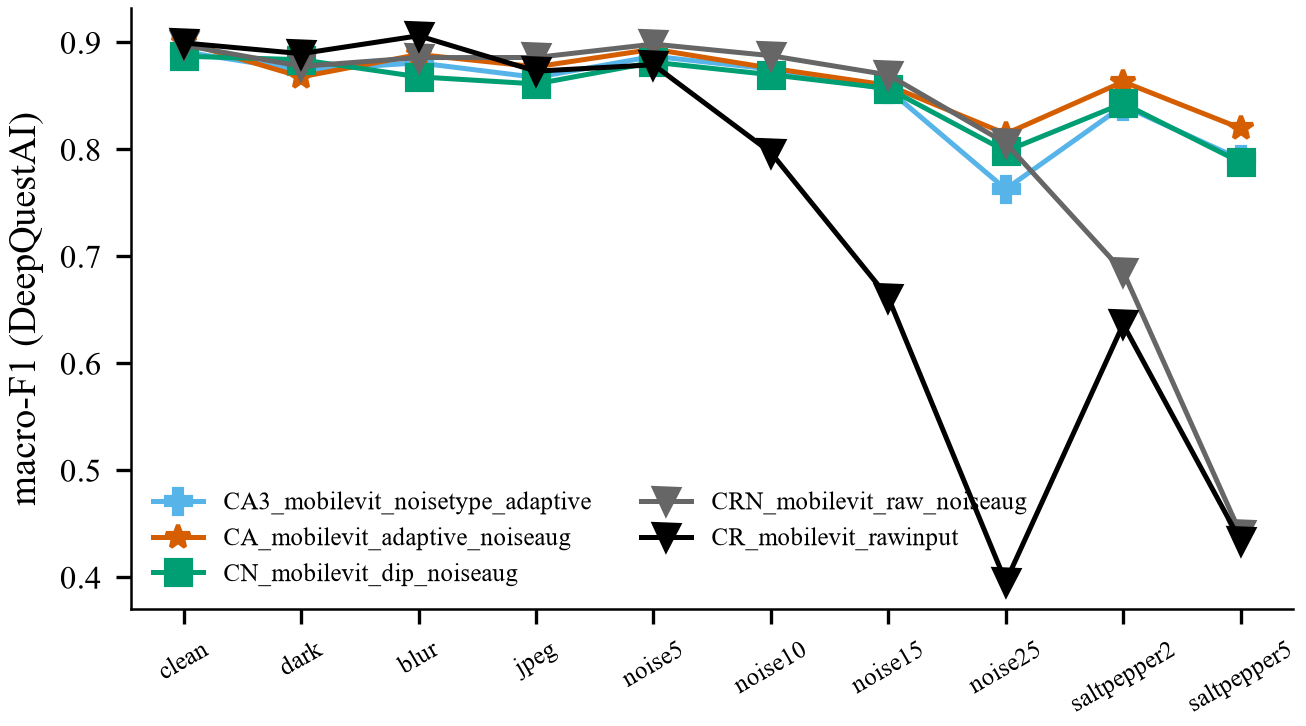
\includegraphics[width=5.20in]{fig25_robust.png}
  \caption{Macro-F1 on DeepQuestAI under each kind of damage. CA2 was tested later in a separate run with the same damage, so it is in Table \ref{tab:robust} but not in this chart.}
  \label{fig:robust}
\end{figure*}

On clean, dark, blurred and JPEG photos the six models are close. The difference appears under noise. CR falls to 0.40 at Gaussian noise of $\sigma$ 25 and to 0.43 at 5\% salt-and-pepper noise. Its fire recall at $\sigma$ 25 is only 0.38, so it misses most fires. CRN has noise training but no filter. It handles Gaussian noise but falls to 0.44 at 5\% salt-and-pepper noise. CN has both the filter and noise training, but it filters clean photos too, and its validation score is the lowest of the MobileViT-XS models. CA and CA2 both stay at 0.81 or higher under every kind of damage. The fire recall at $\sigma$ 25 is 0.91 for CA and 0.906 for CA2. CA2, which also brightens dark photos, is a little better than CA on dark photos (0.877 against 0.868), on JPEG photos and on strong Gaussian noise (0.837 against 0.815 at $\sigma$ 25). The two are almost equal on salt-and-pepper noise. CA2 was still not chosen, because its validation score is lower and it gives more false alarms on look-alike photos. The final model was chosen by validation score only, before these tests were run. An earlier test of model C, which has the filter but no noise training, gave 0.546 at $\sigma$ 25. So both parts are needed: the filter for noisy photos and the noise training.

\subsection{Choosing a filter for each noise type}
Model CA3 first decides the noise type. To find salt-and-pepper noise it counts isolated points with the point mask that has 8 in the centre and $-$1 around it \cite{gonzalez}. A pixel with a response above 600 counts as a lonely dot. CA3 then uses the filter with the best SSIM from Table \ref{tab:e12}. This point detector works poorly once the photo is resized (Section V-G), so the final pipeline does not use it. The corrected model CA3 v2 has a lower validation score than CA and falls to 0.76 at $\sigma$ 25. The filter that gives the best-looking image is not always the best filter for the classifier.


\section{Software Package}
The final model is released as a small Python package named firesmoke. It was built with PyTorch \cite{pytorch}, timm \cite{timm} and OpenCV \cite{opencv}. An export step packs the trained weights, the noise threshold, the filter settings and the class names into one file of about 8 MB. The package uses the same DIP code as the training, so a new photo is treated in the same way as the training photos.

The package can be used in three ways: from the command line, from Python, and from a Google Colab notebook that keeps the model and the results in Google Drive. For every photo it saves the label and the confidence, the measured $\sigma$, the decision (clean or noisy), an image of all steps, a short explanation in words and a file with all numbers. It also saves an image that compares the input with the output of the DIP step, with the PSNR, the SSIM and the share of changed pixels. Fig. \ref{fig:pkg} shows this image for a photo with added noise. For a clean photo the package reports a PSNR of 100 dB, an SSIM of 1.000 and 0\% changed pixels, which shows that clean photos are not touched.

\begin{figure}[H]
  \centering
  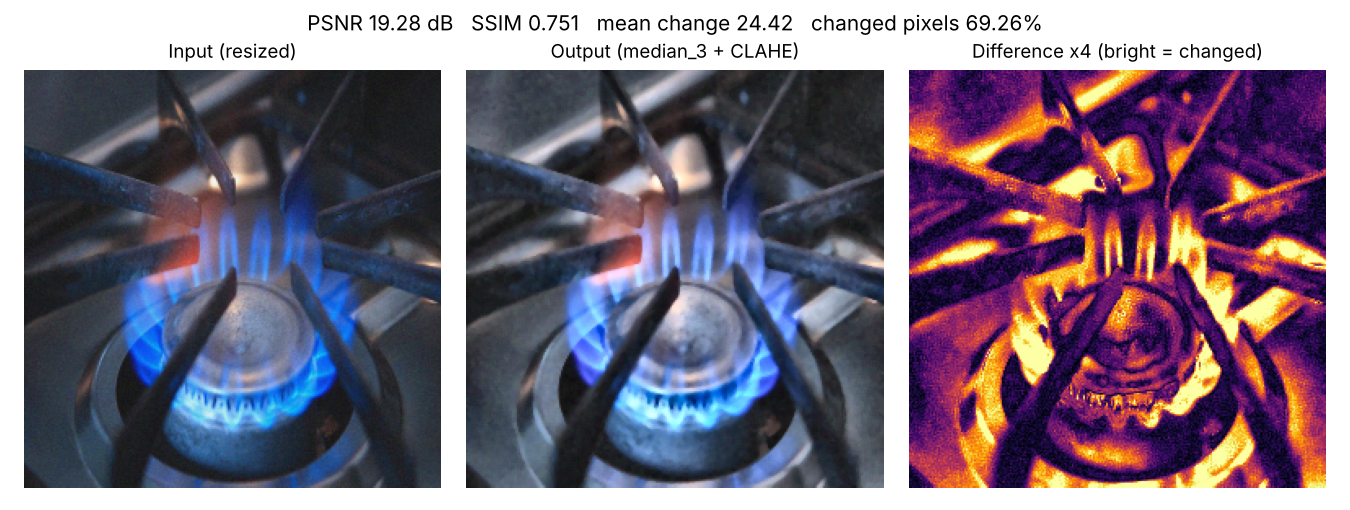
\includegraphics[width=3.50in]{fig26_pkg.png}
  \caption{Input and output comparison saved by the package for a photo with added Gaussian noise. Bright areas in the difference image are the pixels that changed.}
  \label{fig:pkg}
\end{figure}

On the laptop GPU, the model needs about 4.6 ms per photo on the validation set with a batch of 32. In one test on a new photo, a gas stove with a blue flame was called normal with a confidence of 96.1\%. Its noise level was 0.89, so it was not filtered. This answer is useful for an alarm system, because a cooking flame is not a danger. It also shows a limit: the model learned fire as orange and yellow flames.


\section{Discussion}
The results agree with DIP theory \cite{gonzalez}. The median filter is an order-statistic filter. It removes single wrong dots and keeps edges. This is why it is the best filter for salt-and-pepper noise, and why CA does not break on this noise while CR and CRN do.

Every filter also removes some real detail. The median filter alone changes a photo to a PSNR of about 32 dB. The adaptive rule avoids this loss on clean photos. This is why CA is better than C and CN on clean photos.

Global histogram equalisation can stretch flat areas too much and make noise stronger. CLAHE works on small tiles and limits the stretch with a clip limit. Using only the L channel keeps the hue, so the fire colour stays correct.

Area interpolation acts as a low-pass filter. It lowers Gaussian noise and shrinks salt-and-pepper dots. This explains why the isolated point count stopped working when the noise was added before resizing.

The smoke mask is weak because smoke is grey. Sky, fog, roads and walls have the same colour. A colour rule alone cannot separate them. The trained network does much better, because it also uses shape and texture.

Filtering does not remove all noise. Noise training teaches the network to ignore the rest. DIP and deep learning work best together.


\section{Limitations and Future Work}
\begin{itemize}
  \item Each model was trained only once, with one random seed. Small differences between models may be due to chance.
  \item The first filter study added noise after resizing. We corrected it and trained CA3 again. Both results are reported.
  \item The smoke mask marks about 19\% of the area of normal photos.
  \item About 12\% of the normal DeepQuestAI photos are still called fire or smoke.
  \item The brightness rule (CA2) helped only a little on dark photos (0.877 against 0.868 for CA), and it marked 22\% of ordinary photos as dark.
  \item The result folder of model CA2 was deleted by mistake. We tested its saved model again without training and rebuilt its results. Its validation score matched the original run exactly (0.9078).
  \item The system uses single photos. It does not use motion, which is a strong sign of smoke in video.
  \item The model learned fire as orange and yellow flames. Blue flames may be missed.
\end{itemize}

In future work we plan to train every model with several seeds and use paired tests, to add video and motion features, to improve the smoke mask with texture, and to run the package on a small edge device with a camera.


\section{Conclusion}
This work joined classic digital image processing with a small vision transformer for fire and smoke classification. The system measures the noise in each photo and filters only the noisy ones. The final model has the best validation macro-F1 of 16 classifiers (0.917), reaches 0.900 on a test set from a new source and gives false alarms on only 2.2\% of look-alike photos. Under added noise, blur, darkness and JPEG damage it stays at 0.81 or higher, while the same network on raw photos falls to 0.40. The system is available as a Python package that shows every intermediate step.


\balance
\renewcommand{\refname}{References}
\begin{thebibliography}{99}
\footnotesize
\bibitem{muhammad} K. Muhammad, J. Ahmad, and S. W. Baik, ``Early fire detection using convolutional neural networks during surveillance for effective disaster management,'' Neurocomputing, vol. 288, pp. 30--42, 2018.
\bibitem{dodge} S. Dodge and L. Karam, ``Understanding how image quality affects deep neural networks,'' in Proc. 8th Int. Conf. Quality of Multimedia Experience (QoMEX), 2016, pp. 1--6.
\bibitem{hendrycks} D. Hendrycks and T. Dietterich, ``Benchmarking neural network robustness to common corruptions and perturbations,'' in Proc. Int. Conf. Learn. Represent. (ICLR), 2019.
\bibitem{huang} T. S. Huang, G. J. Yang, and G. Y. Tang, ``A fast two-dimensional median filtering algorithm,'' IEEE Trans. Acoust., Speech, Signal Process., vol. 27, no. 1, pp. 13--18, 1979.
\bibitem{clahe} K. Zuiderveld, ``Contrast limited adaptive histogram equalization,'' in Graphics Gems IV, P. S. Heckbert, Ed. San Diego, CA, USA: Academic Press, 1994, pp. 474--485.
\bibitem{immerkaer} J. Immerkær, ``Fast noise variance estimation,'' Comput. Vis. Image Understand., vol. 64, no. 2, pp. 300--302, 1996, doi: 10.1006/cviu.1996.0060.
\bibitem{mobilevit} S. Mehta and M. Rastegari, ``MobileViT: Light-weight, general-purpose, and mobile-friendly vision transformer,'' in Proc. Int. Conf. Learn. Represent. (ICLR), 2022.
\bibitem{chen} T.-H. Chen, P.-H. Wu, and Y.-C. Chiou, ``An early fire-detection method based on image processing,'' in Proc. IEEE Int. Conf. Image Process. (ICIP), 2004, pp. 1707--1710.
\bibitem{toreyin} B. U. Töreyin, Y. Dedeoğlu, U. Güdükbay, and A. E. Çetin, ``Computer vision based method for real-time fire and flame detection,'' Pattern Recognit. Lett., vol. 27, no. 1, pp. 49--58, 2006.
\bibitem{celik} T. Çelik and H. Demirel, ``Fire detection in video sequences using a generic color model,'' Fire Safety J., vol. 44, no. 2, pp. 147--158, 2009, doi: 10.1016/j.firesaf.2008.05.005.
\bibitem{dfire} P. V. A. B. de Venâncio, A. C. Lisboa, and A. V. Barbosa, ``An automatic fire detection system based on deep convolutional neural networks for low-power, resource-constrained devices,'' Neural Comput. Appl., vol. 34, pp. 15349--15368, 2022, doi: 10.1007/s00521-022-07467-z.
\bibitem{catargiu} C. Catargiu, N. Cleju, and I. B. Ciocoiu, ``A comparative performance evaluation of YOLO-type detectors on a new open fire and smoke dataset,'' Sensors, vol. 24, no. 17, Art. no. 5597, 2024, doi: 10.3390/s24175597.
\bibitem{mobilenetv3} A. Howard et al., ``Searching for MobileNetV3,'' in Proc. IEEE/CVF Int. Conf. Comput. Vis. (ICCV), 2019, pp. 1314--1324.
\bibitem{deepquest} DeepQuestAI, ``Fire-Smoke-Dataset,'' GitHub repository. [Online]. Available: https://github.com/DeepQuestAI/Fire-Smoke-Dataset (accessed Nov. 2026).
\bibitem{gonzalez} R. C. Gonzalez and R. E. Woods, Digital Image Processing, 4th ed. New York, NY, USA: Pearson, 2018.
\bibitem{timm} R. Wightman, ``PyTorch image models,'' GitHub repository, 2019, doi: 10.5281/zenodo.4414861.
\bibitem{pytorch} A. Paszke et al., ``PyTorch: An imperative style, high-performance deep learning library,'' in Adv. Neural Inf. Process. Syst., vol. 32, 2019, pp. 8024--8035.
\bibitem{adamw} I. Loshchilov and F. Hutter, ``Decoupled weight decay regularization,'' in Proc. Int. Conf. Learn. Represent. (ICLR), 2019.
\bibitem{he} K. He, J. Sun, and X. Tang, ``Single image haze removal using dark channel prior,'' IEEE Trans. Pattern Anal. Mach. Intell., vol. 33, no. 12, pp. 2341--2353, 2011.
\bibitem{otsu} N. Otsu, ``A threshold selection method from gray-level histograms,'' IEEE Trans. Syst., Man, Cybern., vol. 9, no. 1, pp. 62--66, 1979.
\bibitem{ojala} T. Ojala, M. Pietikäinen, and T. Mäenpää, ``Multiresolution gray-scale and rotation invariant texture classification with local binary patterns,'' IEEE Trans. Pattern Anal. Mach. Intell., vol. 24, no. 7, pp. 971--987, 2002.
\bibitem{haralick} R. M. Haralick, K. Shanmugam, and I. Dinstein, ``Textural features for image classification,'' IEEE Trans. Syst., Man, Cybern., vol. SMC-3, no. 6, pp. 610--621, 1973.
\bibitem{svm} C. Cortes and V. Vapnik, ``Support-vector networks,'' Mach. Learn., vol. 20, no. 3, pp. 273--297, 1995.
\bibitem{rf} L. Breiman, ``Random forests,'' Mach. Learn., vol. 45, no. 1, pp. 5--32, 2001.
\bibitem{efron} B. Efron and R. J. Tibshirani, An Introduction to the Bootstrap. New York, NY, USA: Chapman \& Hall, 1993.
\bibitem{ssim} Z. Wang, A. C. Bovik, H. R. Sheikh, and E. P. Simoncelli, ``Image quality assessment: From error visibility to structural similarity,'' IEEE Trans. Image Process., vol. 13, no. 4, pp. 600--612, 2004.
\bibitem{bilateral} C. Tomasi and R. Manduchi, ``Bilateral filtering for gray and color images,'' in Proc. IEEE Int. Conf. Comput. Vis. (ICCV), 1998, pp. 839--846.
\bibitem{nlm} A. Buades, B. Coll, and J.-M. Morel, ``A non-local algorithm for image denoising,'' in Proc. IEEE Conf. Comput. Vis. Pattern Recognit. (CVPR), 2005, pp. 60--65.
\bibitem{opencv} G. Bradski, ``The OpenCV library,'' Dr. Dobb's J. Softw. Tools, 2000.
\end{thebibliography}

\end{document}